\documentclass[11pt]{article}
\usepackage[margin=1in]{geometry}
\usepackage{amsmath,amssymb}
\usepackage{array,booktabs,longtable,enumitem,xcolor,graphicx,float,subcaption,hyperref,setspace,microtype}
\setstretch{1.10}
\setlength{\emergencystretch}{2em}
% Expected location: repository_root/report/main.tex
% Figures may live in repository_root/figures or report/figures.
\graphicspath{{../figures/}{figures/}}
\hypersetup{colorlinks=true,linkcolor=blue!50!black,urlcolor=blue!50!black,citecolor=black}

\providecommand{\tightlist}{}
\newcommand{\course}{PC5253: Complex Systems Analysis and Modelling}
\newcommand{\semester}{Semester 1, AY2026/2027}
\newcommand{\projecttitle}{Robustness of Knowledge-Graph Retrieval under Network Damage}
\newcommand{\groupid}{G17}

\begin{document}
\begin{center}
{\LARGE\bfseries Group Project Final Report}\\[0.4em]
{\large\bfseries \projecttitle}\\[0.9em]
Group ID: \groupid\\[0.5em]
\course\\
\semester
\end{center}

% INTERNAL NOTE: delete before final submission.
\noindent\fbox{\parbox{\dimexpr\linewidth-2\fboxsep-2\fboxrule\relax}{%
\textbf{Internal writing guide --- delete before submission}
\begin{itemize}[leftmargin=*,itemsep=0.2em,topsep=0.3em]
\item Main report content should be at least \textbf{10 pages}; code, data, and references are excluded.
\item Each member edits only the assigned section file. Avoid editing \texttt{main.tex} unless coordinating the report.
\item Use consistent symbols: damage fraction $f$, structural robustness $S(f)$, and retrieval success $R(f)$ where applicable.
\item Do not hard-code figure/table numbers; use \texttt{\\label} and \texttt{\\ref}.
\item B performs final consistency editing; all members provide key findings, limitations, and takeaways for Section 8.
\end{itemize}}}

\section*{Administrative Information}
\begin{tabular}{@{}>{\bfseries\raggedright\arraybackslash}p{0.25\linewidth}>{\raggedright\arraybackslash}p{0.70\linewidth}@{}}
Group members & Add names and student IDs. \\[0.7em]
Project area & Complex networks, knowledge graphs, percolation, and retrieval robustness. \\[0.7em]
Repository & \url{https://github.com/zzy0304Raymond/pc5253-g17-primekg} \\
\end{tabular}

\tableofcontents
\clearpage

\section{Introduction}
\label{sec:introduction}

\subsection{Why the question matters}

Knowledge graphs store facts as typed links between entities. In biomedicine,
PrimeKG links drugs, diseases and proteins \cite{chandak2023primekg}. Such a
graph is used by following short paths. Drug-repurposing methods score a drug
for a disease by the proteins the two share, or by how close the drug's targets
lie to the disease proteins in the interaction network
\cite{guney2016network}. Retrieval-augmented language models answer questions
from the neighborhood of a few hops around the entities in the question
\cite{edge2024graphrag}. In both uses, a fact is useful only if a short path to
it survives.

Real knowledge graphs lose links all the time, through incomplete curation,
retracted findings, or a data source that drops out of a merge. Their health is
usually judged with global statistics, chief among them the size of the giant
component. This is the quantity that network robustness studies track under
random failure and targeted attack \cite{albert2000error,callaway2000network}.
We ask whether that statistic tells us anything about the short paths that
applications actually use.

\subsection{The answer in one figure}

Figure~\ref{fig:summary} answers the question on a 5,000-node sample of PrimeKG
and a fixed benchmark of 200 drug--disease queries. Each query asks whether a
drug and a disease are still linked through a shared protein within $L$ hops.
Panel~(a) removes edges at random. With half of the edges gone, 98\% of nodes
are still in the giant component and 86\% of queries can still be reached by a
path of any length, but only 41\% keep a two-hop answer. Panel~(b) removes 5\%
of nodes, either at random or by targeting the highest-degree or
highest-betweenness nodes. The attacks cost the giant component 6--7
percentage points more than random removal, but they cost two-hop retrieval
57--63 points more. The giant component therefore misses most of the functional
damage, and it understates the extra harm of targeted damage by nearly an order
of magnitude.

\begin{figure}[!htbp]
  \centering
  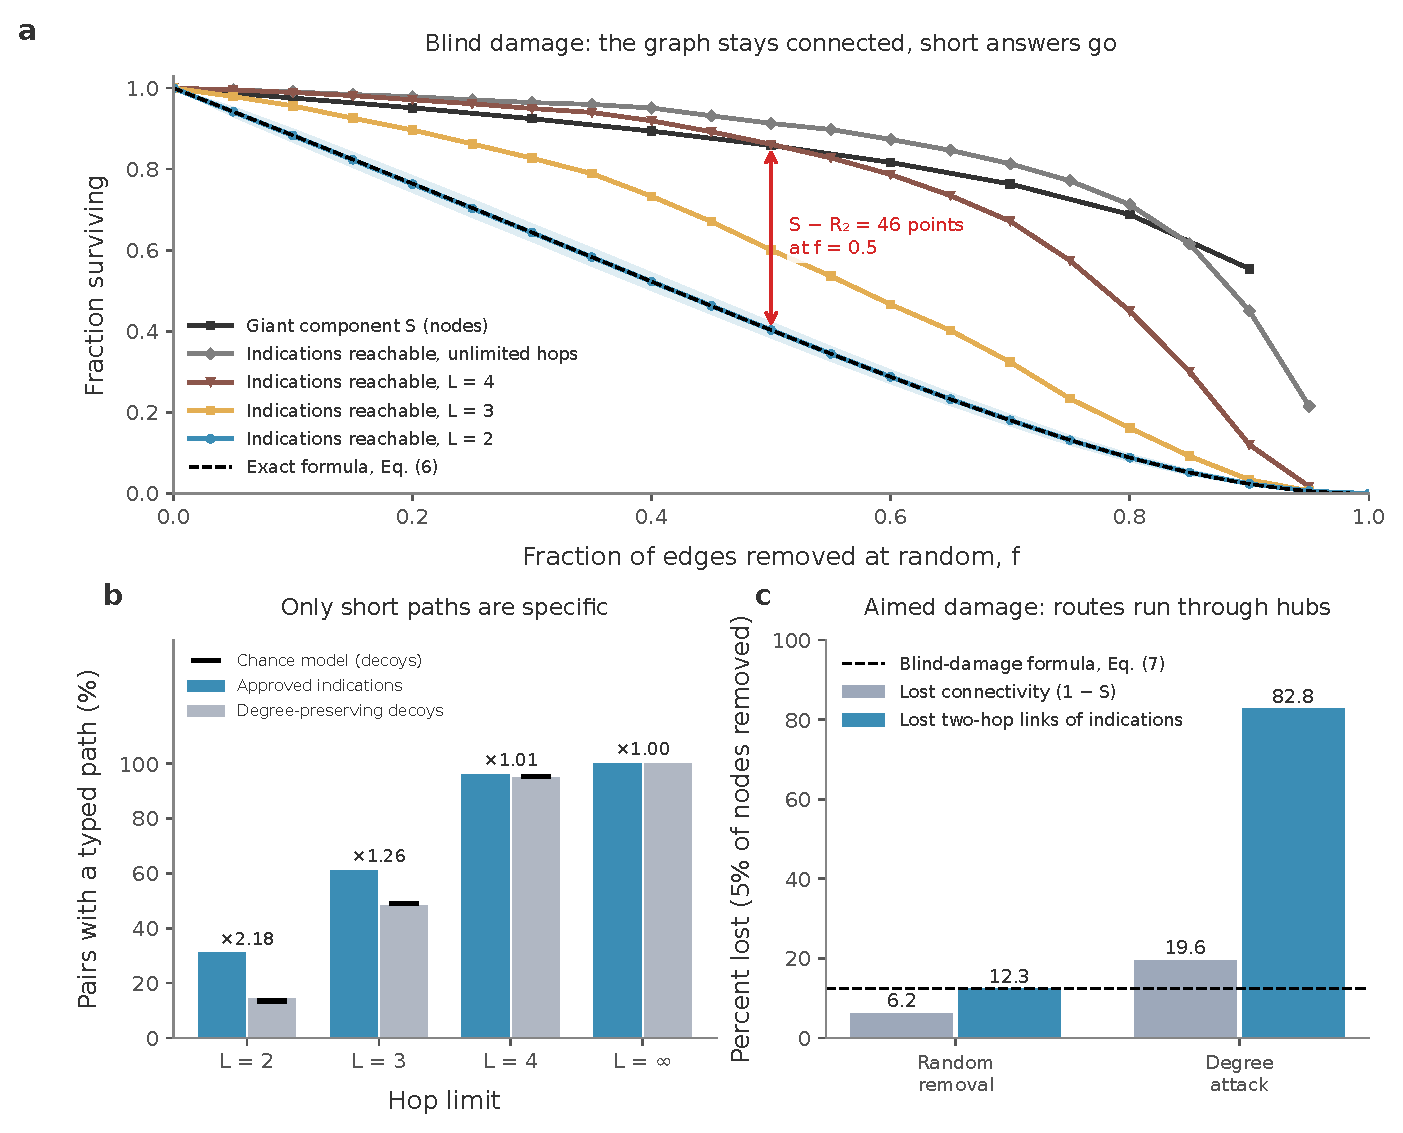
\includegraphics[width=\linewidth]{act0/fig_summary.pdf}
  \caption{The main results. (a) Random edge removal: giant component $S$
  (mean of ten damage orders) and retrieval success $R_L$ with hop limit $L$
  (mean of 600 independent damage orders). Shading shows the spread of a single
  damage state (one standard deviation). Dashed lines are the predictions of
  Section~\ref{sec:theory}, which contain no fitted parameters. (b) Damage after
  removing 5\% of nodes at random (mean of ten orders) or by a fixed degree or
  betweenness ranking. The dashed line shows the two-hop loss expected if the
  same number of nodes were removed blindly.}
  \label{fig:summary}
\end{figure}

\subsection{What explains it}

The course treated connectivity with generating functions and percolation. We
show that one simple principle covers connectivity and retrieval together. A
quantity survives damage if at least one of its redundant units survives, so
its survival probability is one minus the generating function of its redundancy
distribution, evaluated at the failure probability of one unit
(Section~\ref{sec:theory}). The three curves in Figure~\ref{fig:summary}a
differ because they use different units and different redundancy
distributions:
\begin{itemize}[leftmargin=*,itemsep=1pt]
\item nodes have a median of 25 edges, and only 2\% have a single edge;
\item the median query has a minimum cut of 6 edges between its drug and its
disease, and 22\% have a cut of one;
\item half of the queries have exactly one shared protein.
\end{itemize}
The principle is exact for two-hop retrieval under blind damage and
approximate for the other two. It also makes clear where it must fail: when
damage is aimed at hubs, because many of the redundant units of a query sit on
hubs.
Most of the gap between $S$ and $R_2$ is due to the hop limit, not to
fragmentation of the graph.

\subsection{Contributions}

\begin{enumerate}[leftmargin=*,itemsep=2pt]
\item \textbf{A common description.} We describe connectivity, unlimited-hop
reachability and bounded-hop retrieval as the same expression with three
different redundancy distributions. We separate what is exact from what is
approximate, and we test every approximation against independent simulations.
\item \textbf{An explanation of the gap.} At 50\% edge loss, needing both
endpoints to stay attached costs 12 points, and the two-hop limit costs a
further 45. Longer horizons move the bottleneck from shared proteins to drug
target links.
\item \textbf{An account of targeted damage.} Attacks violate the assumption
that every unit survives with the same probability. A degree-resolved version of
the formula reproduces the attacked retrieval rate, and we split the loss into
lost endpoints and lost routes. We use degree-preserving null models to attribute the excess structural
fragility, and we check the result on the full filtered graph.
\item \textbf{A consequence for repair.} The two-hop formula predicts the gains
of random and relation-type repair without fitting. Through the relation
types that two-hop routes use, it also explains why restoring drug and disease
links is the best policy we tested for two-hop retrieval at large budgets.
\end{enumerate}

\subsection{Beyond the course}

Lectures 6--9 developed percolation on random graphs and on interdependent
networks. Four ideas in this report go beyond that material.
\begin{itemize}[leftmargin=*,itemsep=2pt]
\item Bounded-hop observables are reliability polynomials, in the sense of
Moore and Shannon \cite{moore1956reliable}. They have no threshold, unlike the
giant component. Limited-path percolation \cite{lopez2007limited} describes
the regime between the two.
\item Degree-preserving null models at increasing levels of constraint
\cite{maslov2002specificity} can attribute the failure of generating-function
theory on a real network to specific structure.
\item Path count is not effective redundancy. Under targeted damage what matters
is the degree of the node each route passes through.
\item Correlated test items reduce effective sample size. Because queries share
drug links, 200 queries behave like about 90 independent ones.
\end{itemize}
A typed query needs an edge in each of two relation layers, drug--protein and
disease--protein. It is therefore a small multiplex object, in the sense of
Lecture~9, and the best repair policy turns out to be layer-aware.

Section~\ref{sec:data} describes the data, benchmark and damage model, and
Section~\ref{sec:theory} develops the theory. Sections~\ref{sec:blind}
and~\ref{sec:targeted} test it under blind and targeted damage,
Section~\ref{sec:repair} applies it to repair, and Section~\ref{sec:discussion}
separates what generalizes from what is specific to our sample.

\section{Data, Queries and Damage}
\label{sec:data}

\subsection{The graph}
\label{sec:data-graphs}

We use a fixed release of PrimeKG \cite{chandak2023primekg}
(file \texttt{kg.csv}, Harvard Dataverse file 6180620; checksums in
Appendix~\ref{app:repro}). We keep three entity types (drug, disease,
gene/protein) and three relations (drug--protein, disease--protein,
protein--protein). Reverse and duplicate records are merged into one undirected
edge per entity pair, and self-loops are removed. This filtered graph, which we
call the full graph, has 30,968 nodes and 426,954 edges. No entity pair carries
more than one relation, so the routes between a drug and a disease through
different proteins share no edge, which Section~\ref{sec:theory-r2} uses.

\subsection{Queries: approved indications and decoys}
\label{sec:data-indications}

A query $(d,y)$ asks whether drug $d$ and disease $y$ are linked through
proteins. It succeeds at hop limit $L$ if there is a typed path
\begin{equation*}
d \xrightarrow{\text{drug--protein}} x_1 \xrightarrow{\text{PPI}} \cdots
\xrightarrow{\text{PPI}} x_j \xrightarrow{\text{disease--protein}} y,
\qquad j-1\le L-2,
\end{equation*}
with $j-1$ protein--protein (PPI) steps. For $L=2$ the drug and disease must share
a protein, and the number $m$ of shared proteins is the query's redundancy
(Figure~\ref{fig:schematic}).

\begin{figure}[!htbp]
  \centering
  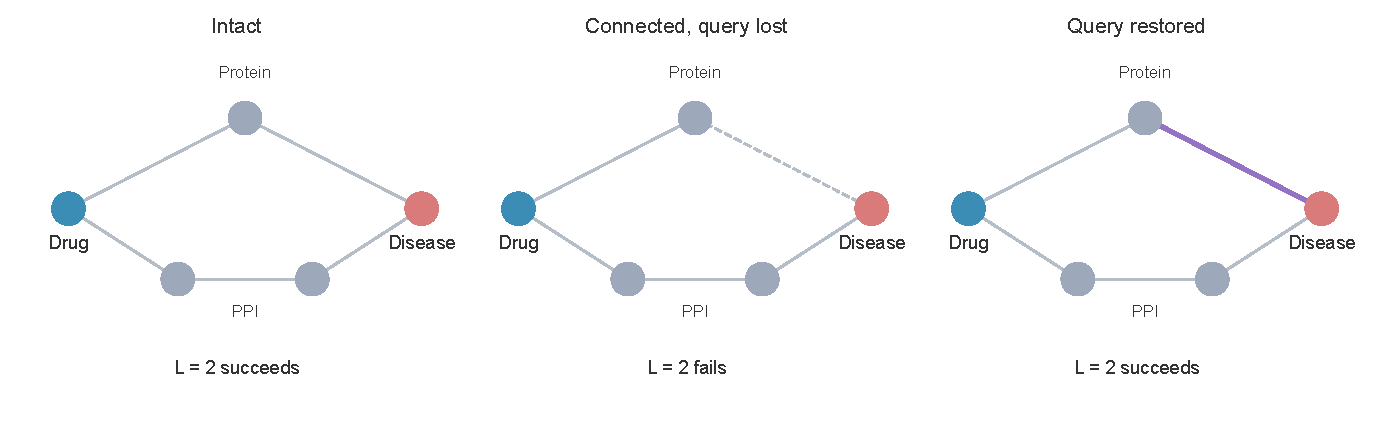
\includegraphics[width=0.86\linewidth]{act0/fig_query_schematic.pdf}
  \caption{A typed query. Left: the drug and the disease share a protein, so the
  query succeeds at $L=2$; a longer route through two interacting proteins also
  exists. Middle: losing one disease--protein link leaves the pair connected, but
  the two-hop answer is gone, which is the situation of this report's title.
  Right: restoring that link recovers it (Appendix~\ref{sec:repair}).}
  \label{fig:schematic}
\end{figure}

The main queries are PrimeKG's approved drug indications. PrimeKG lists 9,388
drug--disease indication pairs, and for 6,233 of them both endpoints are in the
full graph. These pairs are not part of the graph we damage, because only
drug--protein, disease--protein and protein--protein edges were kept, so they
are evidence that the retrieval rule has not seen. For each indication we form a
decoy by permuting the diseases among the indicated drugs and rejecting any pair
that PrimeKG lists as an indication, a contraindication or an off-label use.
Every decoy keeps the drug of one indication and the decoy diseases are the
indicated diseases in a new order, so the two sets have almost identical
distributions of drug and disease degree. We report the recall (the share of
indications with a typed path within $L$ hops), the decoy rate (the same share
for decoys), their ratio, and the mutual information in bits between the label
and the retrieval outcome for a balanced mixture of the two sets. Of the
indications, 1,931 have at least one shared protein; we call them two-hop
indications. Our first benchmark drew its queries from the graph we were
damaging, so it could tell us whether paths survive but not whether they mean
anything. Indications that the damaged graph does not contain turned a
robustness exercise into the question of this report.

\subsection{A controlled testbed}
\label{sec:data-sample}

To test the theory under full control, we also use the induced subgraph on the
first 5,000 nodes reached by breadth-first search (BFS) from the disease of
highest degree, with ties broken by index, which we call the sample. Its
benchmark has 200 drug--disease queries that succeed at $L=2$: 100 with $m=1$
and 100 with $m\ge2$, drawn with a fixed seed from the 3,175 and 1,264 such
pairs. They involve 39 drugs and 127 diseases. The 50/50 mix sets the level of
$R_2$, so the benchmark's success rates describe this controlled task, not
PrimeKG. Table~\ref{tab:graphs} compares the two graphs.

\begin{table}[!htbp]
\centering
\small
\caption{Graphs used in this report. Assortativity $r$ is the degree
correlation across edges \cite{newman2002assortative}. The last column is the mean degree of the neighbors of nodes with degree at most 3, averaged over
their edges. For an uncorrelated graph with the same degrees it would be
$\langle k^2\rangle/\langle k\rangle$, which is 189 for the sample and 190 for the full graph.}
\label{tab:graphs}
\begin{tabular}{@{}lrrrrrrrr@{}}
\toprule
Graph & Nodes & Edges & Drugs & Diseases & Proteins & $\langle k\rangle$ & $r$ & Neighbor degree \\
\midrule
BFS sample & 5,000 & 117,891 & 74 & 283 & 4,643 & 47.2 & $-0.153$ & 486 \\
Full graph & 30,968 & 426,954 & 6,282 & 5,593 & 19,093 & 27.6 & $-0.053$ & 209 \\
\bottomrule
\end{tabular}
\end{table}

The sample has 90,187 protein--protein, 27,228 disease--protein and
only 476 drug--protein edges. Proteins make up 93\% of its nodes. Of its 74
drugs, 51 have a single target.

\paragraph{The sample is not PrimeKG.} BFS reaches peripheral nodes through
hubs, and a node at the frontier keeps only its edges into nodes already
visited. The sample therefore has a denser core than the full graph, and its
low-degree nodes hang from hubs. Table~\ref{tab:graphs} shows this directly. In
the full graph, low-degree nodes have neighbors only slightly more connected
than in an uncorrelated graph (209 against 190), and the assortativity is
$-0.053$. In the sample these values are 486 and $-0.153$. The sample's median
degree is 25 and only 2\% of its nodes have a single edge; in the full graph
these are 9 and 22\%. The sample is therefore a testbed for the theory, not a
model of PrimeKG, and we state which conclusions concern it only.

\subsection{Damage and observables}
\label{sec:data-damage}

Under blind damage, a fraction $f$ of edges or nodes is removed in a random
order; removing a node also removes its edges. We write $p=1-f$ for edge
retention and $\phi=1-f$ for node retention. For targeted damage, nodes are
removed in decreasing order of degree, or of betweenness centrality estimated
from 100 sampled sources (seed 42); both rankings are computed once on the
intact graph. The giant component $S(f)$ is the share of the original nodes in
the largest connected component. Retrieval success $R_L(f)$ is the share of
queries that still have a typed path of at most $L$ hops; a query whose drug or
disease has been removed fails.

Expected values under blind damage are Monte Carlo means over independent damage
orders: on the sample, 5,000 orders when two-hop retrieval is compared with
Eq.~\eqref{eq:r2} and 600 for scans over the hop limit; on the full graph, 500
orders for the two-hop indications of Figure~\ref{fig:summary}a and five orders
for all other scans, including the comparisons of all indications with decoys. Ten fixed orders (seeds 0--9) are used
where a stored damage state is needed and to show the spread of a single damage
state. Each order is a random permutation, and the damage state at fraction $f$
is its first $\mathrm{round}(fE)$ entries. Targeted removal is deterministic.

\section{Theory}
\label{sec:theory}
% Owner: D. Target: about 2 pages.
% GF percolation, PGF retrieval formula, L -> infinity limit, limited-path percolation.
\textit{[D: present the theoretical framework and notation here.]}


\section{Structural Robustness}
\label{sec:structural}
\subsection{Structural Robustness under Random Failure}
\label{sec:random-failure}

\subsubsection{Simulation and theoretical
reference}\label{simulation-and-theoretical-reference}

We compute all removal states by reversing each fixed removal order and
adding edges or nodes with a union-find structure, following the
reverse-addition approach of Newman--Ziff \cite{newman2000efficient}. Each returned array
is indexed by the number removed. For semantic duplicates on one
endpoint pair, connectivity changes only when the first surviving
relation is added. This implementation yields largest-component size,
component count and isolated-node count, together with surviving
structural and semantic edge counts.

We compare the curves with a generating-function prediction based on the
original empirical structural degree distribution. Define
$g_0(z)=\sum_k p_k z^k$ and $g_1(z)=g_0'(z)/g_0'(1)$. For edge retention
$q$, the reference solves $u=1-q+qg_1(u)$, taking the nontrivial solution
where it exists. Bond robustness is $1-g_0(u)$; site robustness under node
retention $q$ is $q[1-g_0(u)]$. We use the actual retained fraction after
integer rounding. These are configuration-model approximations, not exact
identities for a finite, typed biological network. Fixed-count deletion
also differs slightly from independent Bernoulli retention at finite size.

\subsubsection{Standard-graph results}\label{standard-graph-results}

The 5,000-node graph is initially connected. Under random edge removal,
most nodes remain in its largest component even after substantial
relation loss. At f=0.50, mean S is 0.98218 with sample SD 0.00128. At
f=0.90, it is 0.81540 $\pm$ 0.00366, and at f=0.99 it falls to 0.11222 $\pm$
0.01592. Thus the largest component remains large over much of the
sampled damage range but loses most original nodes at extreme edge
removal.

\begin{longtable}[]{@{}lrrrr@{}}
\caption{Random-failure robustness on the 5,000-node graph.}\label{tab:a-random}\\
\toprule\noalign{}
Removal & f & Mean S & Sample SD & GF reference \\
\midrule\noalign{}
\endhead
\bottomrule\noalign{}
\endlastfoot
Edge & 0.50 & 0.98218 & 0.00128 & 0.98213 \\
Edge & 0.90 & 0.81540 & 0.00366 & 0.81431 \\
Edge & 0.99 & 0.11222 & 0.01592 & 0.12578 \\
Node & 0.50 & 0.49252 & 0.00345 & 0.49106 \\
Node & 0.90 & 0.08474 & 0.00351 & 0.08143 \\
\end{longtable}

Figure~\ref{fig:a-random} shows the random edge and node curves with their configuration-model references.

\begin{figure}[htbp]
\centering
\begin{subfigure}[t]{0.49\linewidth}
\centering
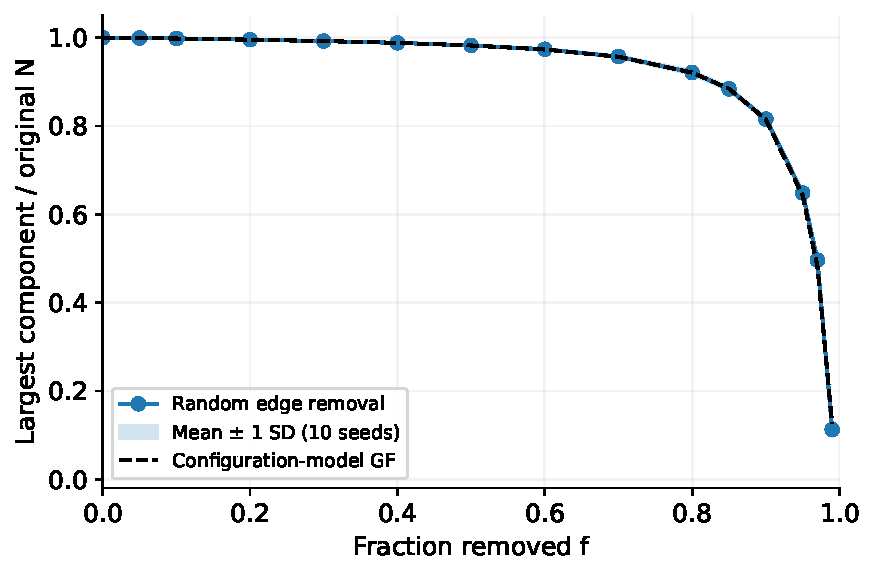
\includegraphics[width=\linewidth]{a_random_edge.pdf}
\caption{Edge removal.}
\end{subfigure}\hfill
\begin{subfigure}[t]{0.49\linewidth}
\centering
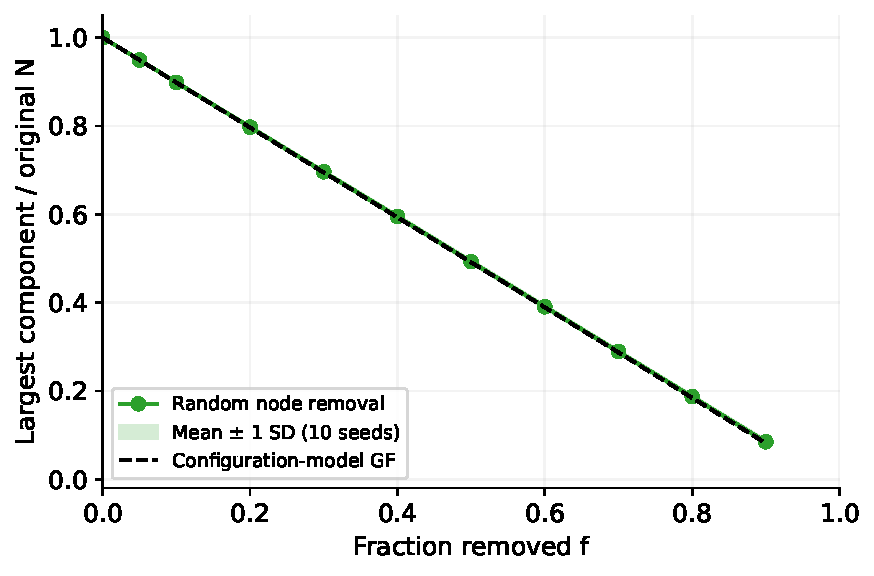
\includegraphics[width=\linewidth]{a_random_node.pdf}
\caption{Node removal.}
\end{subfigure}
\caption{Random-failure simulations on the 5,000-node graph; shading is the sample SD across ten seeds and dashed curves are configuration-model references.}
\label{fig:a-random}
\end{figure}

Under random node removal, S declines almost proportionally to the
surviving fraction over much of the range. At f=0.50, S$\approx$0.49252 means
about 98.5\% of surviving nodes belong to the largest component. A lower
node-removal curve than edge-removal curve does not by itself show
greater fragmentation at equal damage cost: deleted nodes directly
reduce the numerator and remove multiple incident edges. The fixed N0
denominator and additional surviving-edge counts make this distinction
explicit.

The GF reference tracks the main curves closely, with a more noticeable
bond difference at extreme removal. This is a quantitative observation
for this graph and these sample sizes, not proof that the network
satisfies configuration-model assumptions. We do not assign a unique
structural cause to the residual without further controls. The finite
graph and discrete damage grid also do not support an exact universal
critical threshold from curve shape alone.

\subsubsection{Sampling sensitivity and full-graph
comparison}\label{sampling-sensitivity-and-full-graph-comparison}

The filtered full graph gives a materially different bond curve. At
f=0.50, mean S$\approx$0.85830, compared with 0.98218 in the 5,000-node BFS
graph, a difference of approximately 0.124. At f=0.90, the corresponding
values are 0.55382 and 0.81540. These comparisons use the same damage
definition and ten seeds, but the graphs have different compositions and
permutation realizations; they are not paired measurements of identical
physical failures.

The full-graph result shows that the BFS subgraph overstates retention
of original nodes in the largest component for these damage levels.
Protein-rich sampling, degree changes and the removal of peripheral
parts of the full network are plausible contributors, but this
experiment alone does not isolate their separate effects. We therefore
present the 5,000-node curves as results for the agreed standard
subgraph and use the full graph to constrain claims about PrimeKG more
broadly. Figure~\ref{fig:a-sampling} displays this comparison.

\begin{figure}[htbp]
\centering
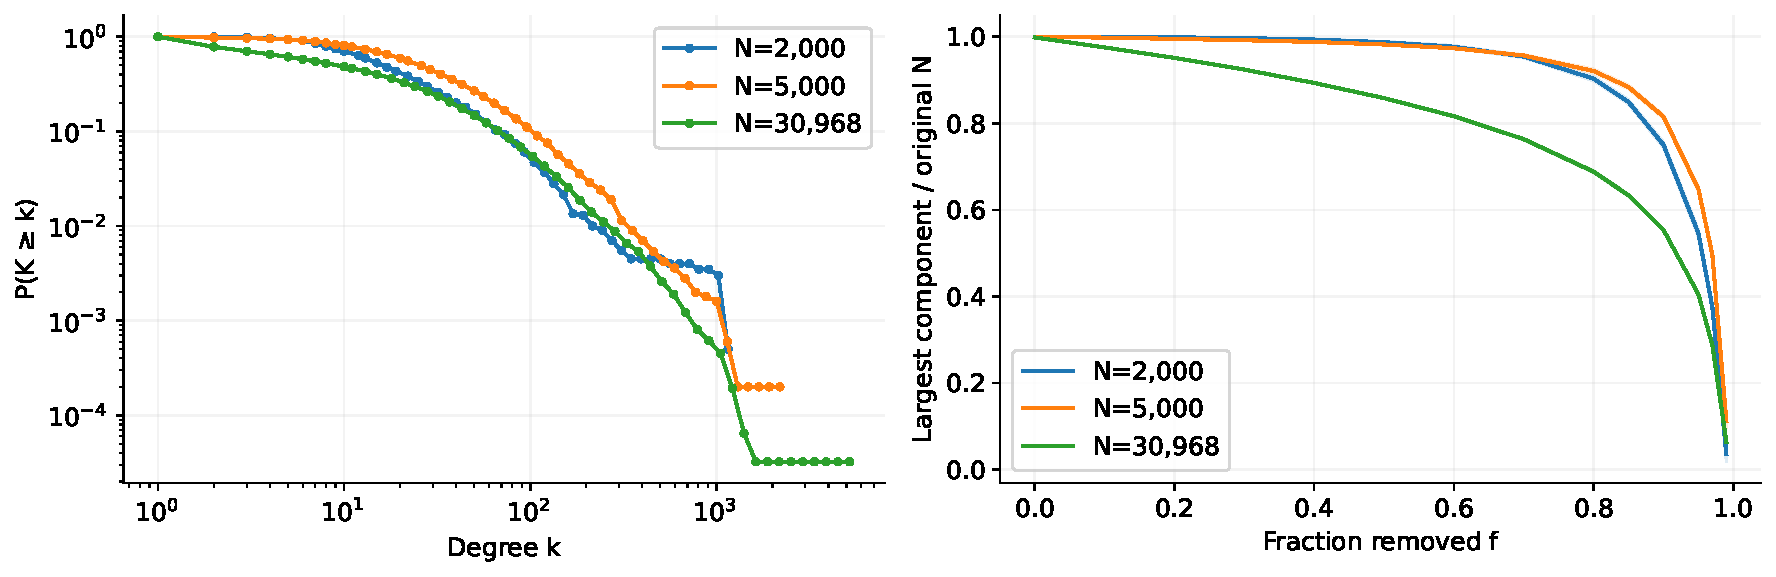
\includegraphics[width=0.82\linewidth]{a_sampling_comparison.pdf}
\caption{Random-edge robustness in the BFS samples and filtered full graph. The different graph constructions limit generalization from the 5,000-node sample.}
\label{fig:a-sampling}
\end{figure}

\subsubsection{Validation and connection to subsequent
workstreams}\label{validation-and-connection-to-subsequent-workstreams}

The union-find implementation was compared with independent NetworkX
calculations at every deletion state on 80 small random graphs,
including empty graphs and repeated semantic endpoint pairs. For each
real graph, independent checks at f=0, 0.3, 0.5, 0.9 and 1 cover both
edge and node deletion and six structural counts. The GF solver passes
the analytic 3-regular configuration-model identity. Separately, a clean
Python 3.11.9 rebuild reproduces all 68 core scientific
graph/query/order files byte-for-byte, including the shared BFS prefix.

For downstream retrieval and restoration, reference fixtures contain
endpoint survival, surviving two-hop path counts and PPI distances at
the same seed-0 damage states. They are computed independently with
NetworkX and can be used to validate C's retriever and E's zero-budget
baseline. The independent fixtures are distinct from the later C and E
integration checks documented elsewhere in the repository. This foundation allows the
subsequent sections to ask whether a structurally large component still
supports the fixed semantic tasks, and whether attacks or restoration
alter that relationship.

\subsection{Targeted Attacks and Null-Model Comparison}
\label{sec:targeted-attacks}

Random-failure experiments treat all nodes as equally likely to fail. However, nodes in a knowledge graph can differ substantially in their structural importance. A node connected to many other entities may act as a hub, while another node may connect otherwise weakly linked regions of the graph. We therefore ask how vulnerable the PrimeKG network is when structurally important nodes are deliberately removed first. We compare random node removal with two targeted strategies based on degree and betweenness centrality on the same 5,000-node PrimeKG subgraph.

\subsubsection{Centrality-Based Attack Strategies}
For a node $v$, its degree is
\begin{equation}
    k_v = \deg(v),
\end{equation}
which is the number of nodes directly connected to $v$. Nodes with high degree therefore act as local hubs with many direct connections. A degree-based attack removes nodes in decreasing order of degree.

Betweenness centrality instead measures how frequently a node lies on shortest paths between other nodes. For node $v$,
\begin{equation}
C_B(v)=\sum_{s\neq v\neq t}\frac{\sigma_{st}(v)}{\sigma_{st}},
\end{equation}
where $\sigma_{st}$ is the number of shortest paths between $s$ and $t$, and $\sigma_{st}(v)$ is the number of those paths that pass through $v$. Degree therefore emphasizes local connectivity, whereas betweenness emphasizes bridge or bottleneck roles.

For both targeted strategies, centrality scores are computed once on the intact graph and the resulting rankings are kept fixed throughout the experiment. The attack sequence is therefore a fixed original ranking rather than an adaptive strategy that recomputes centrality after every removal.

We quantify structural robustness using the giant connected component (GCC) fraction
\begin{equation}
S(f)=\frac{|\mathrm{GCC}(f)|}{N_0},
\end{equation}
where $f$ is the fraction of nodes removed, $|\mathrm{GCC}(f)|$ is the number of surviving nodes in the largest connected component, and $N_0$ is the original number of nodes. Because the denominator is fixed at the original graph size, directly removed nodes also count as lost.

\subsubsection{Robustness under Targeted Node Removal}
Figure~\ref{fig:ws2-attacks} compares random node failure with degree- and betweenness-based attacks. Targeted attacks consistently leave a smaller giant component than random removal. At $f=0.20$, random failure retains approximately 79.7\% of the original graph in the GCC, whereas degree and betweenness attacks retain approximately 69.0\% and 68.6\%, respectively. At $f=0.50$, the difference is substantially larger: $S_{\mathrm{random}}\approx0.493$, $S_{\mathrm{degree}}\approx0.232$, and $S_{\mathrm{betweenness}}\approx0.206$.

\begin{figure}[H]
    \centering
    % Repository path expected: figures/ws2_attack_curves_primekg_5000_bfs_v1.png
    \IfFileExists{../figures/ws2_attack_curves_primekg_5000_bfs_v1.png}{%
      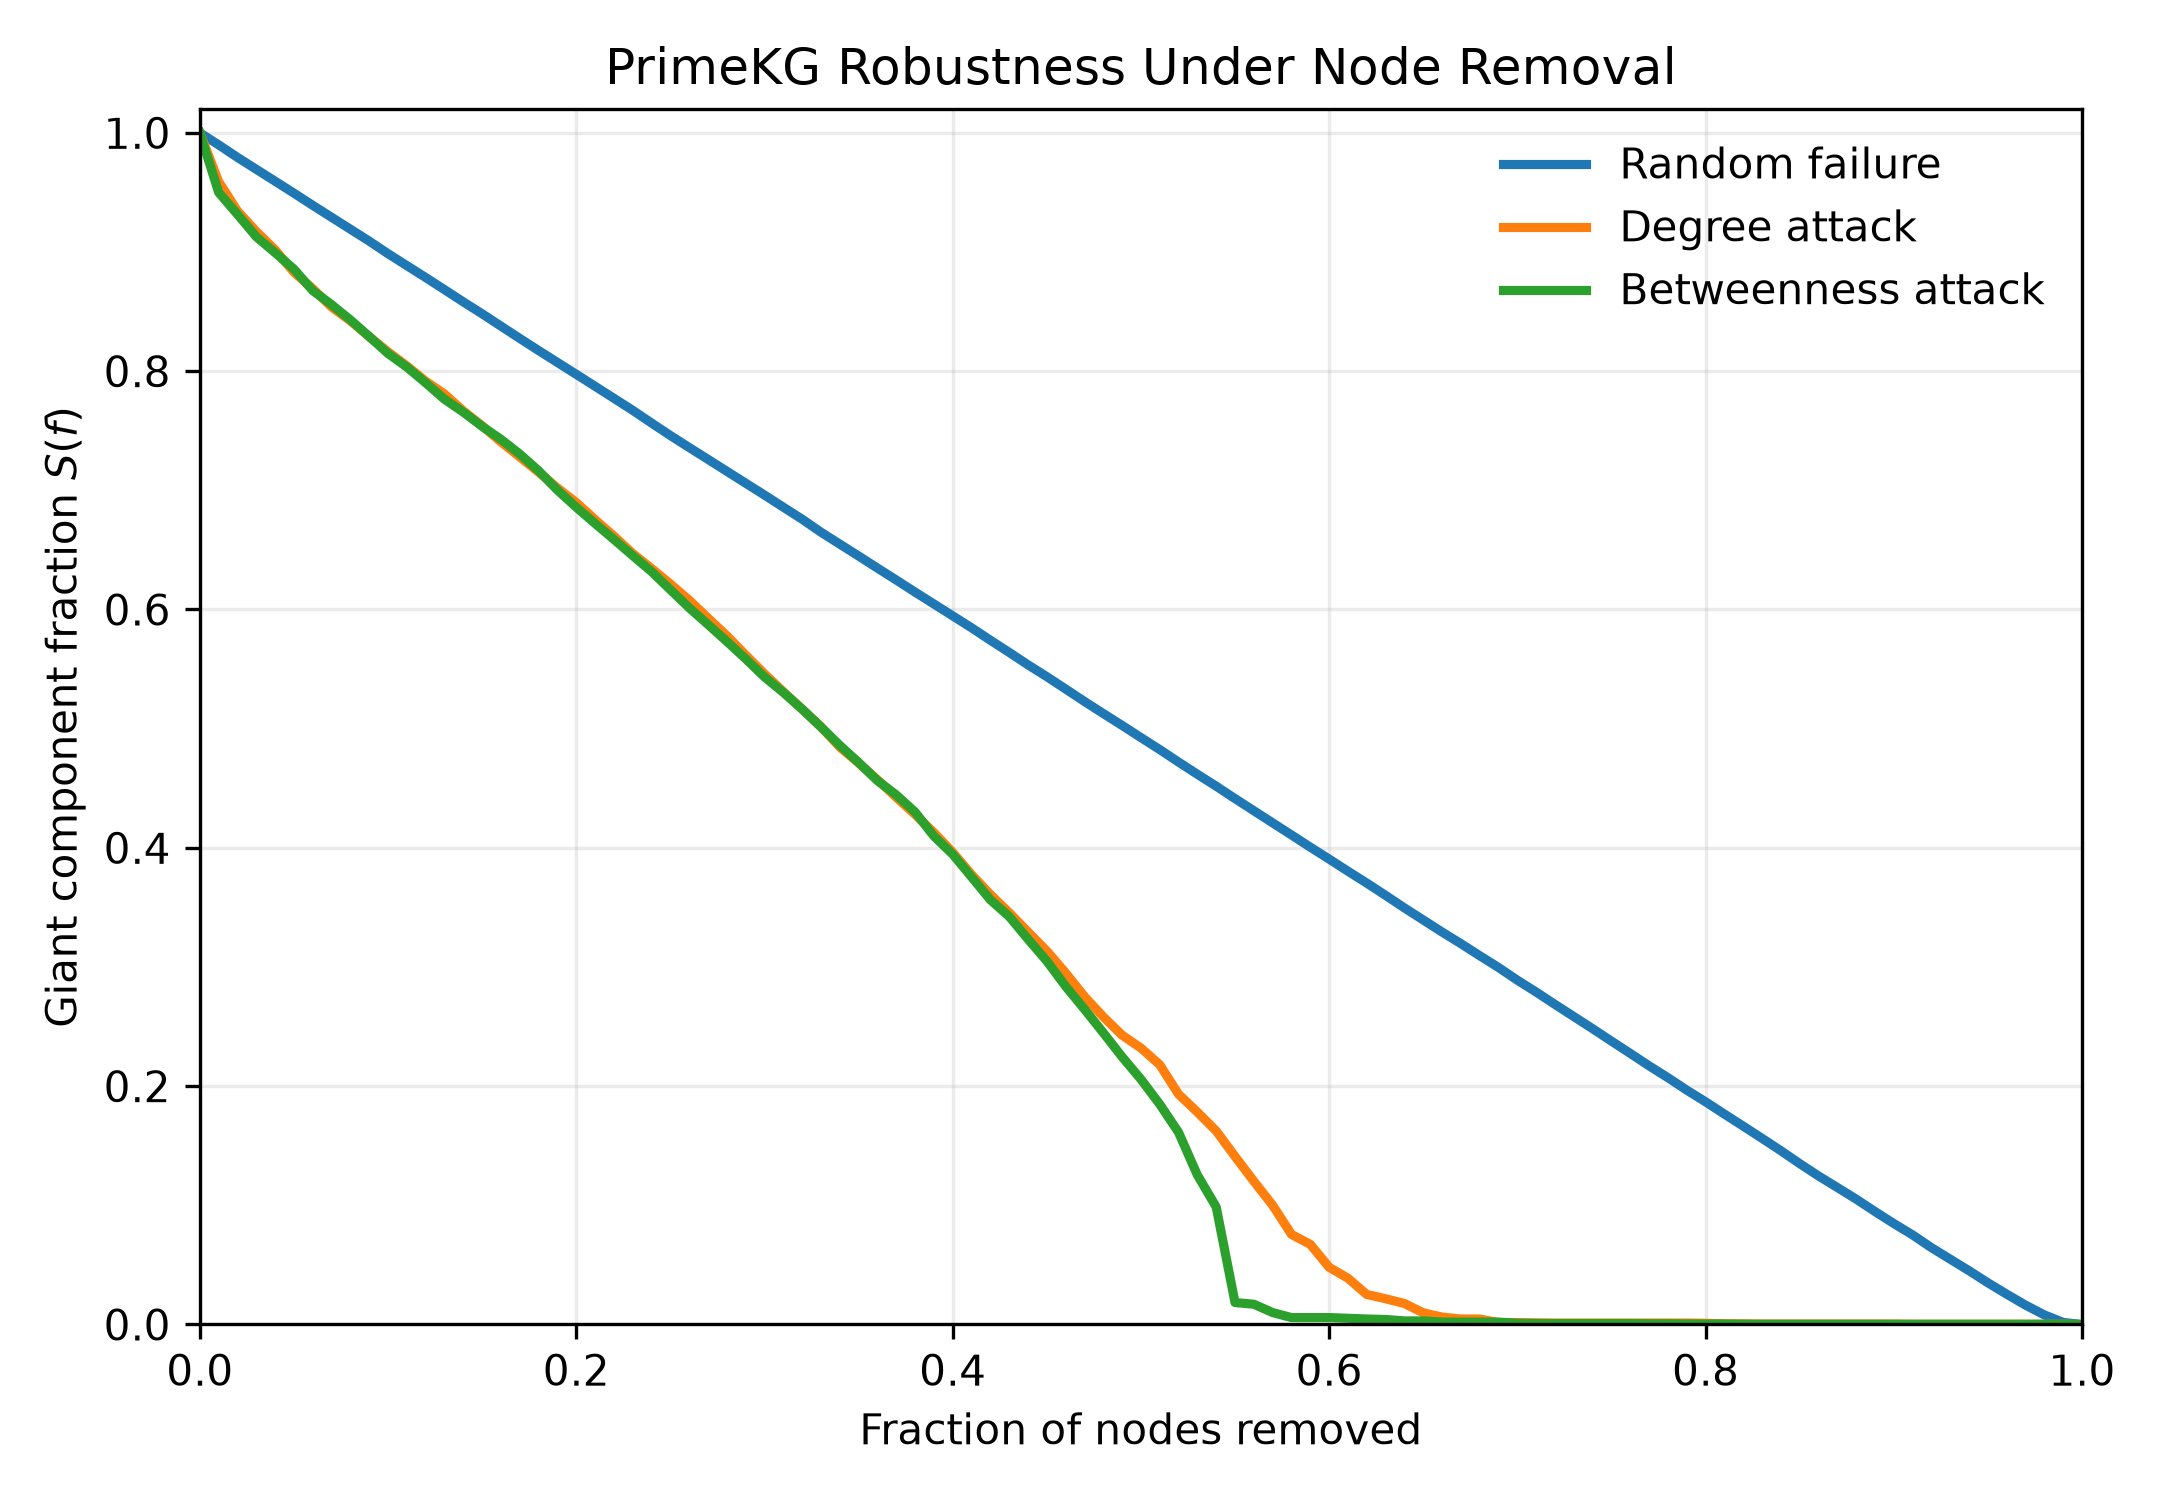
\includegraphics[width=0.86\linewidth]{ws2_attack_curves_primekg_5000_bfs_v1.png}%
    }{%
      \IfFileExists{figures/ws2_attack_curves_primekg_5000_bfs_v1.png}{%
        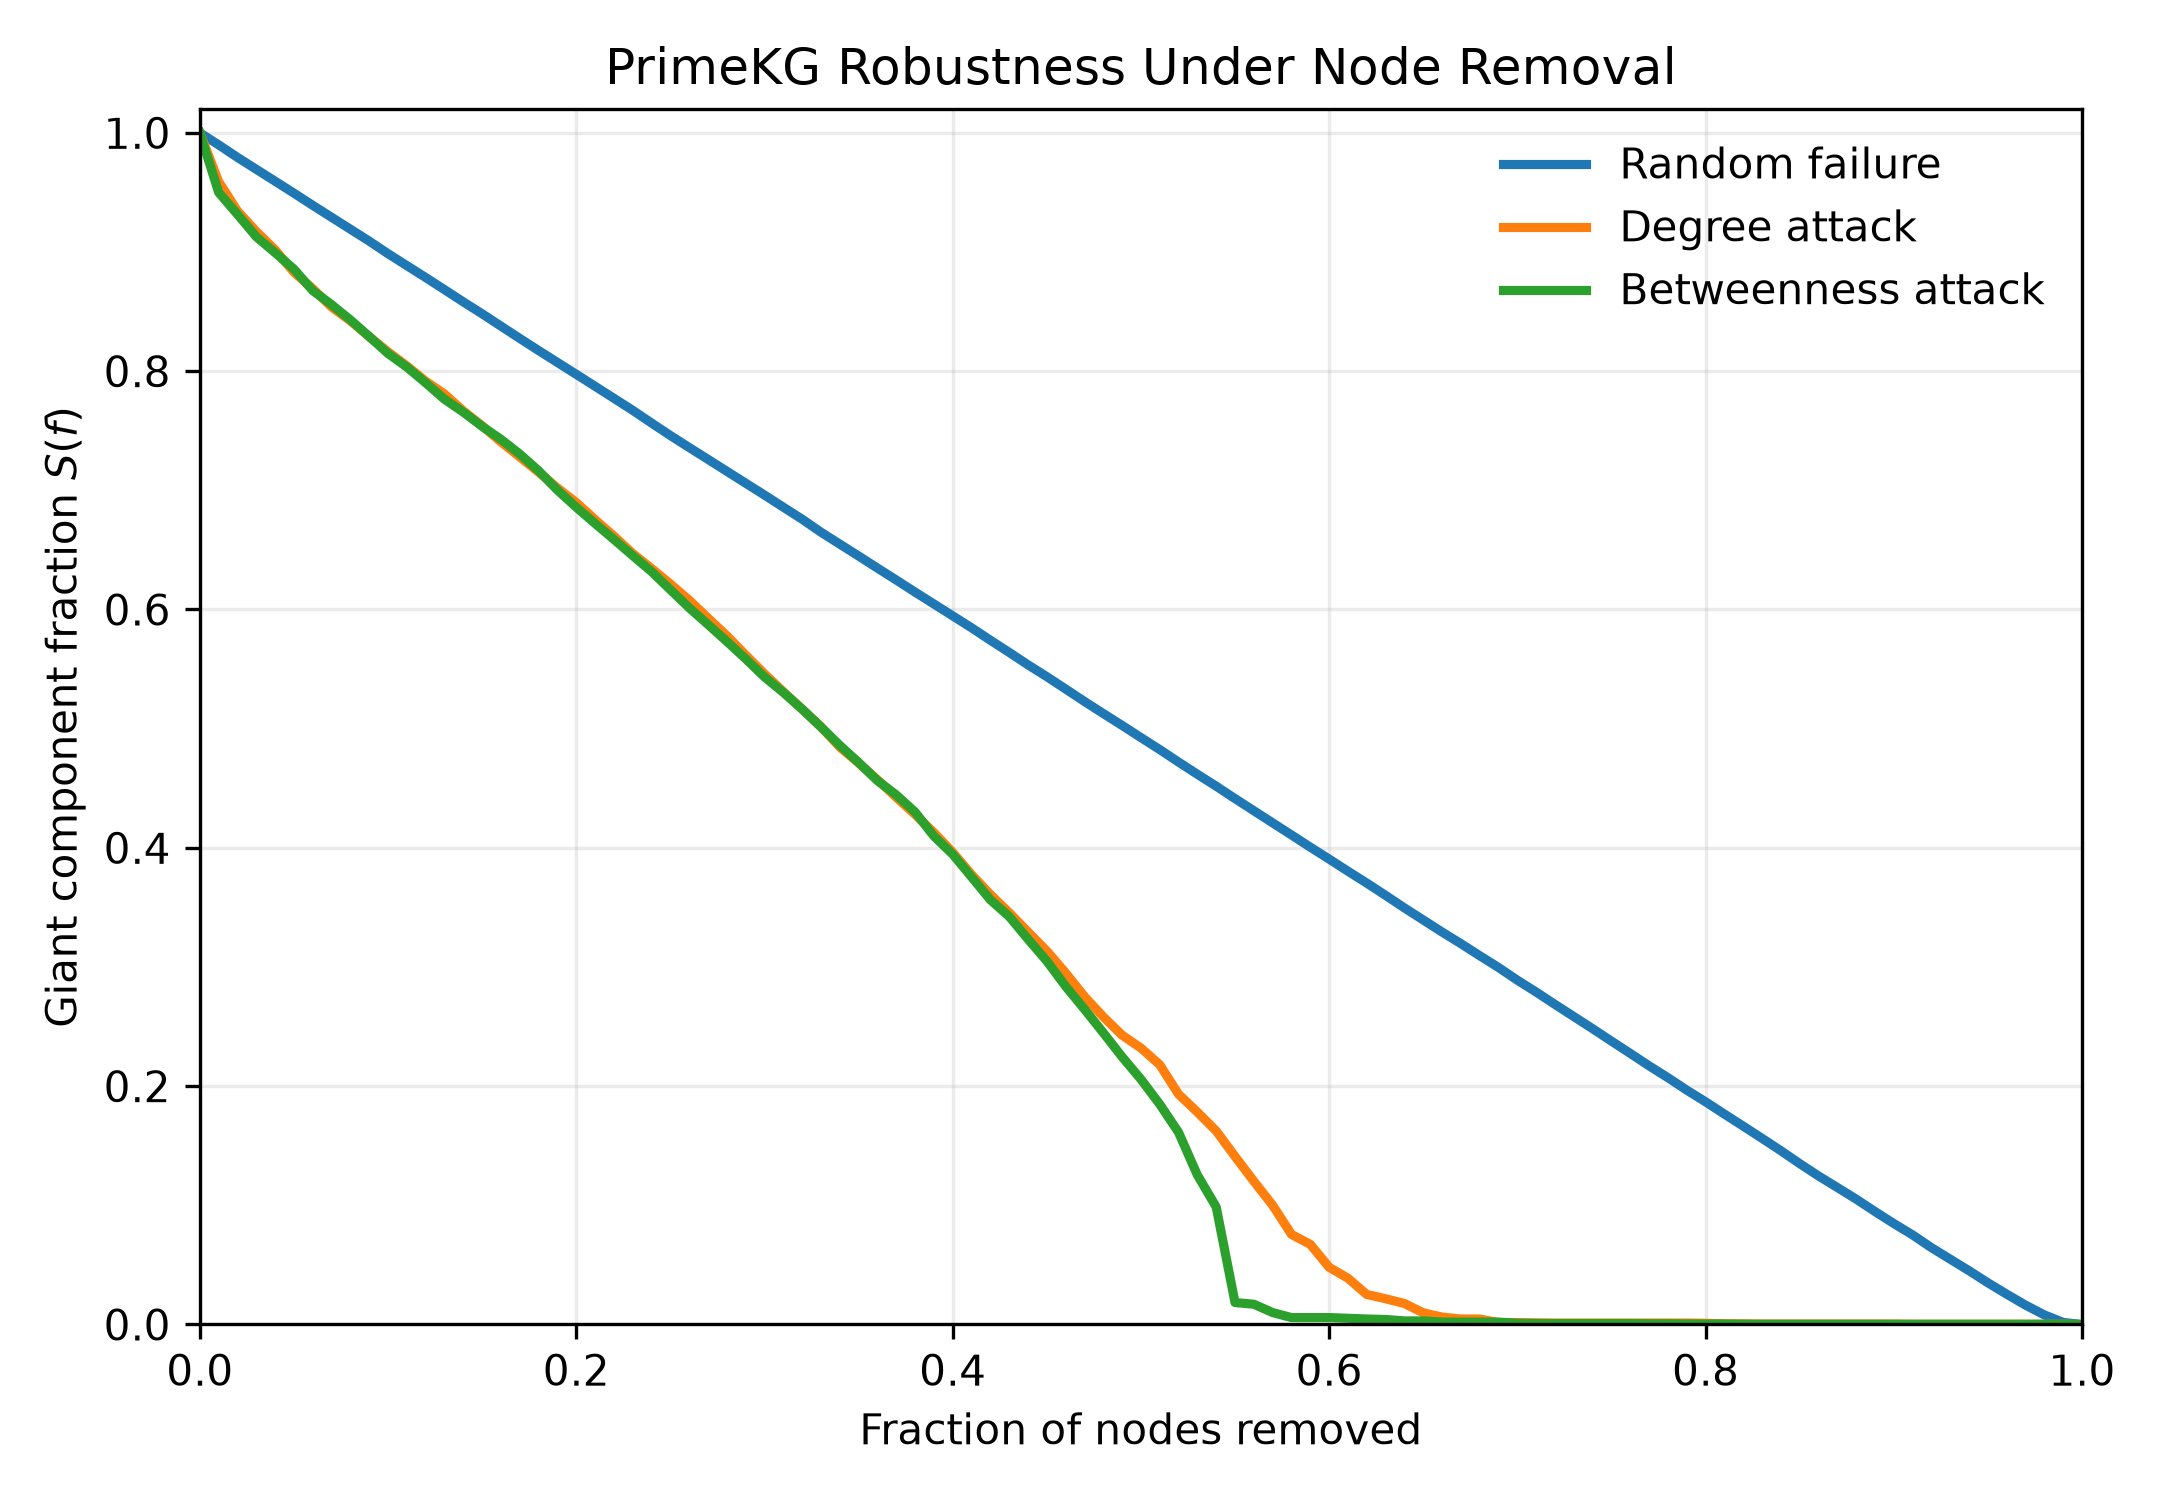
\includegraphics[width=0.86\linewidth]{ws2_attack_curves_primekg_5000_bfs_v1.png}%
      }{%
        \fbox{\parbox[c][2.2in][c]{0.82\linewidth}{\centering Placeholder: WS2 targeted-attack curve\\\texttt{figures/ws2\_attack\_curves\_primekg\_5000\_bfs\_v1.png}}}%
      }%
    }
    \caption{Structural robustness under random and targeted node removal. Degree and betweenness rankings are computed on the intact graph and kept fixed.}
    \label{fig:ws2-attacks}
\end{figure}

\begin{table}[H]
\centering
\caption{Selected GCC fractions under random and targeted node removal.}
\label{tab:ws2-gcc}
\begin{tabular}{@{}lccc@{}}
\toprule
Fraction removed & Random failure & Degree attack & Betweenness attack \\
\midrule
0.20 & 0.797 & 0.690 & 0.686 \\
0.50 & 0.493 & 0.232 & 0.206 \\
\bottomrule
\end{tabular}
\end{table}

These results show that robustness to random failure does not imply robustness to targeted failure. The PrimeKG subgraph is considerably more vulnerable when node removal is concentrated on structurally important entities. The similar behavior of the two targeted strategies also motivates examining whether the two centrality measures identify the same critical nodes.

\subsubsection{Composition and Overlap of Central Nodes}
The 5,000-node graph contains 4,643 gene/protein nodes, 283 disease nodes, and 74 drug nodes. Disease nodes therefore represent only $283/5000=5.66\%$ of the graph overall. However, within the top 1\% of the degree ranking, 16\% are disease nodes; within the top 1\% of the betweenness ranking, 14\% are disease nodes. Disease entities are therefore over-represented among structurally central nodes relative to their overall frequency in the graph.

\begin{figure}[H]
    \centering
    \IfFileExists{../figures/ws2_degree_hub_composition_primekg_5000_bfs_v1.png}{%
      \begin{subfigure}{0.48\linewidth}
      \centering
      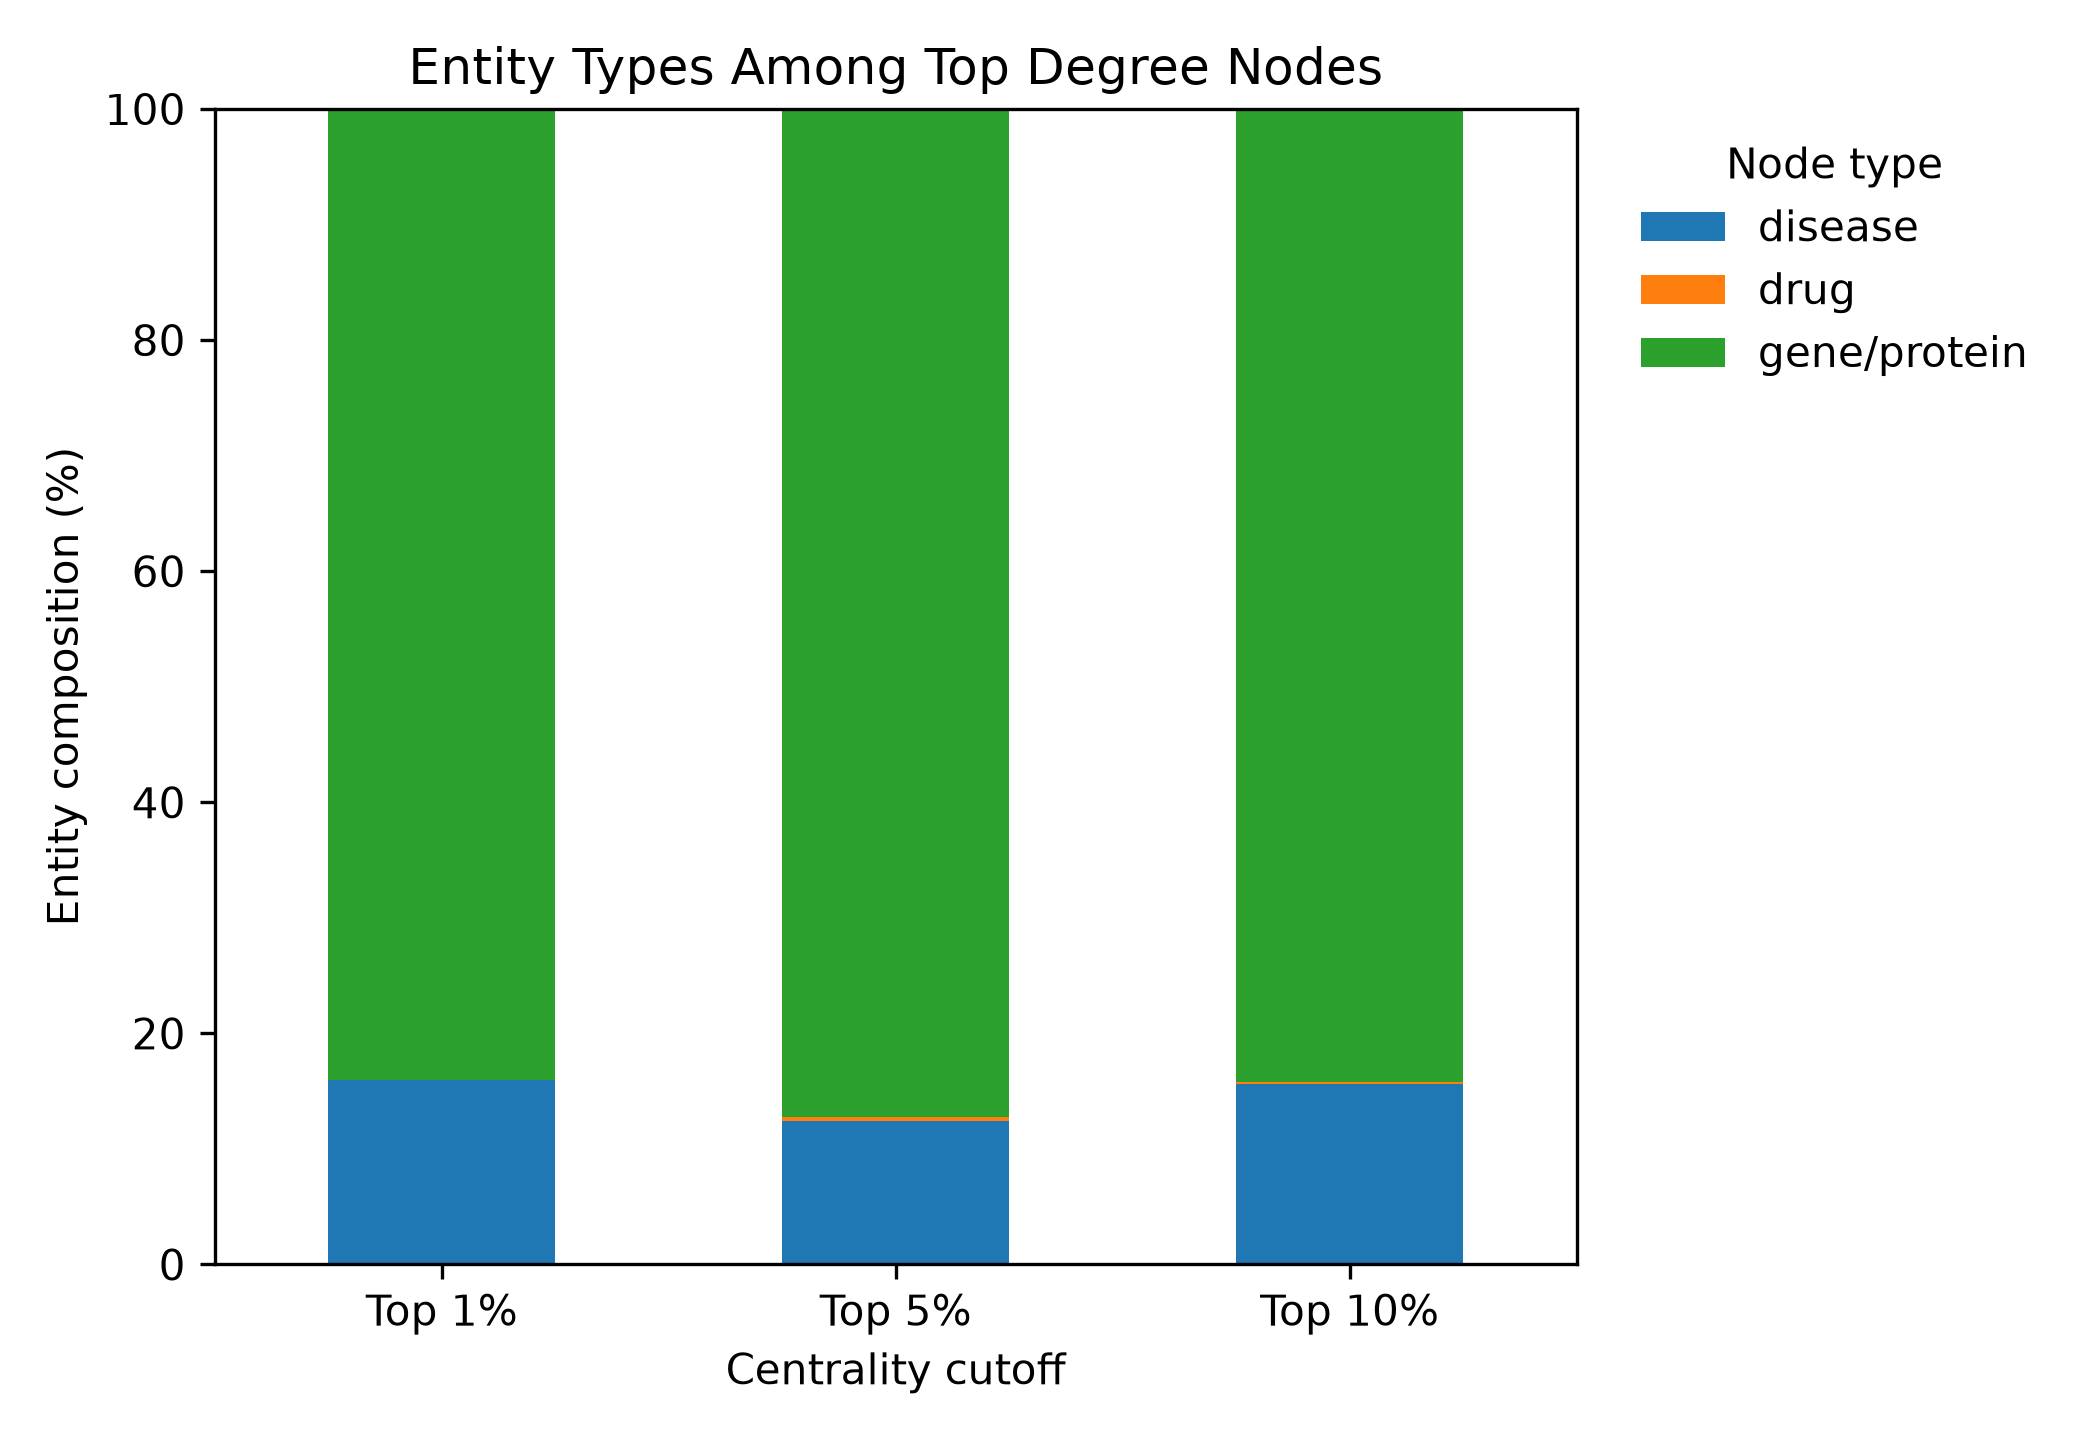
\includegraphics[width=\linewidth]{ws2_degree_hub_composition_primekg_5000_bfs_v1.png}
      \caption{Degree ranking}
      \end{subfigure}\hfill
      \begin{subfigure}{0.48\linewidth}
      \centering
      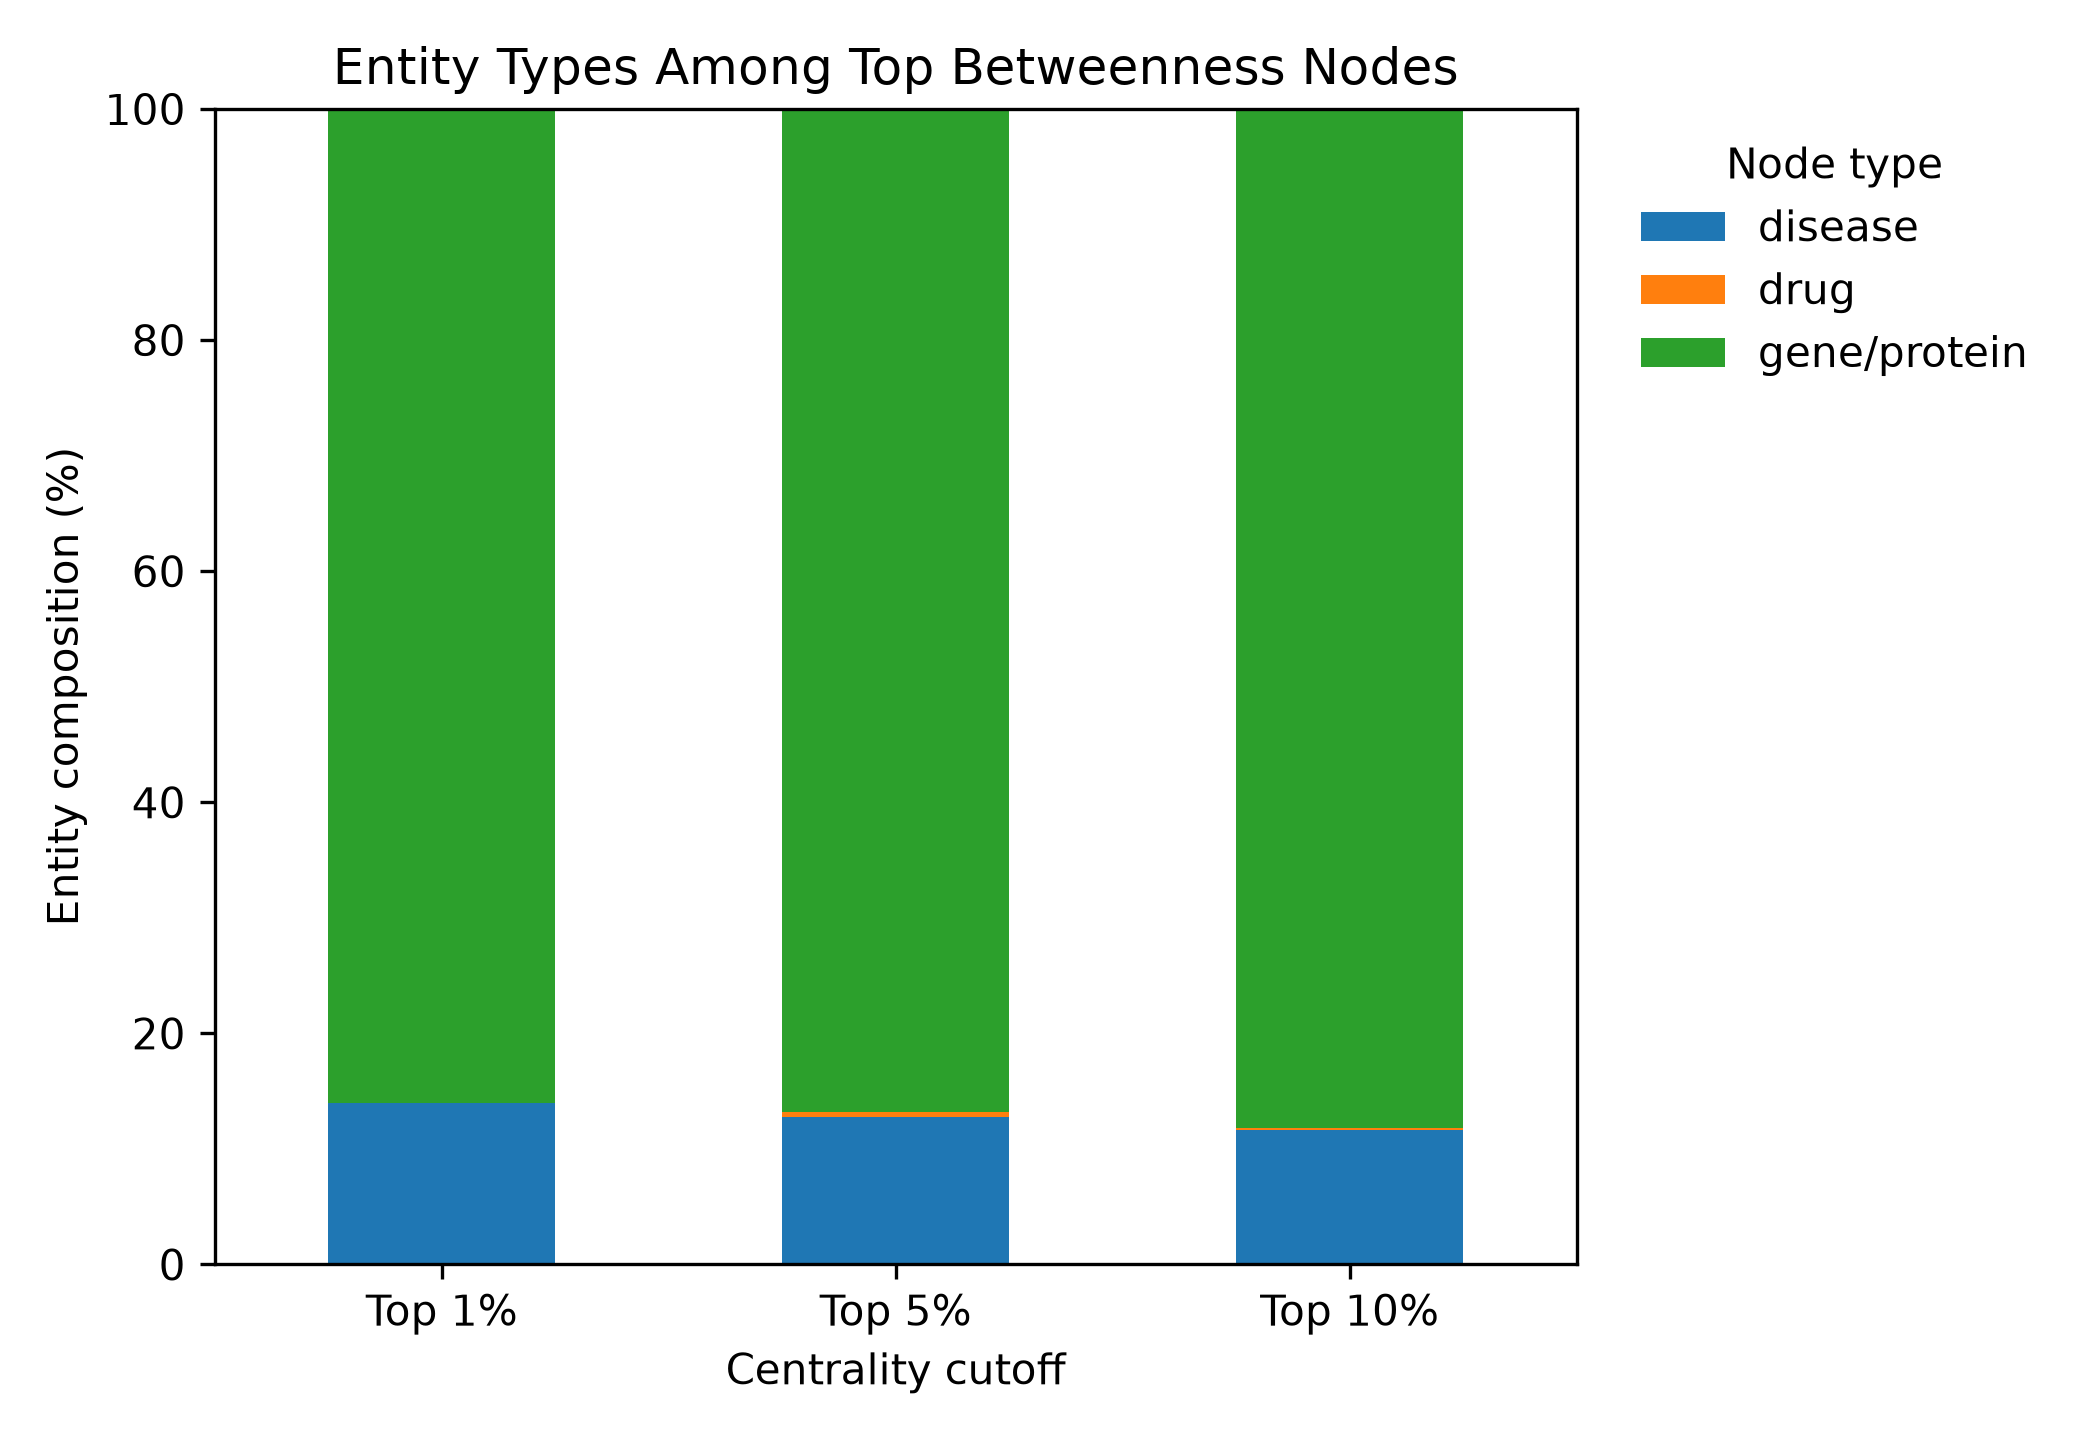
\includegraphics[width=\linewidth]{ws2_betweenness_hub_composition_primekg_5000_bfs_v1.png}
      \caption{Betweenness ranking}
      \end{subfigure}
    }{%
      \IfFileExists{figures/ws2_degree_hub_composition_primekg_5000_bfs_v1.png}{%
      \begin{subfigure}{0.48\linewidth}
      \centering
      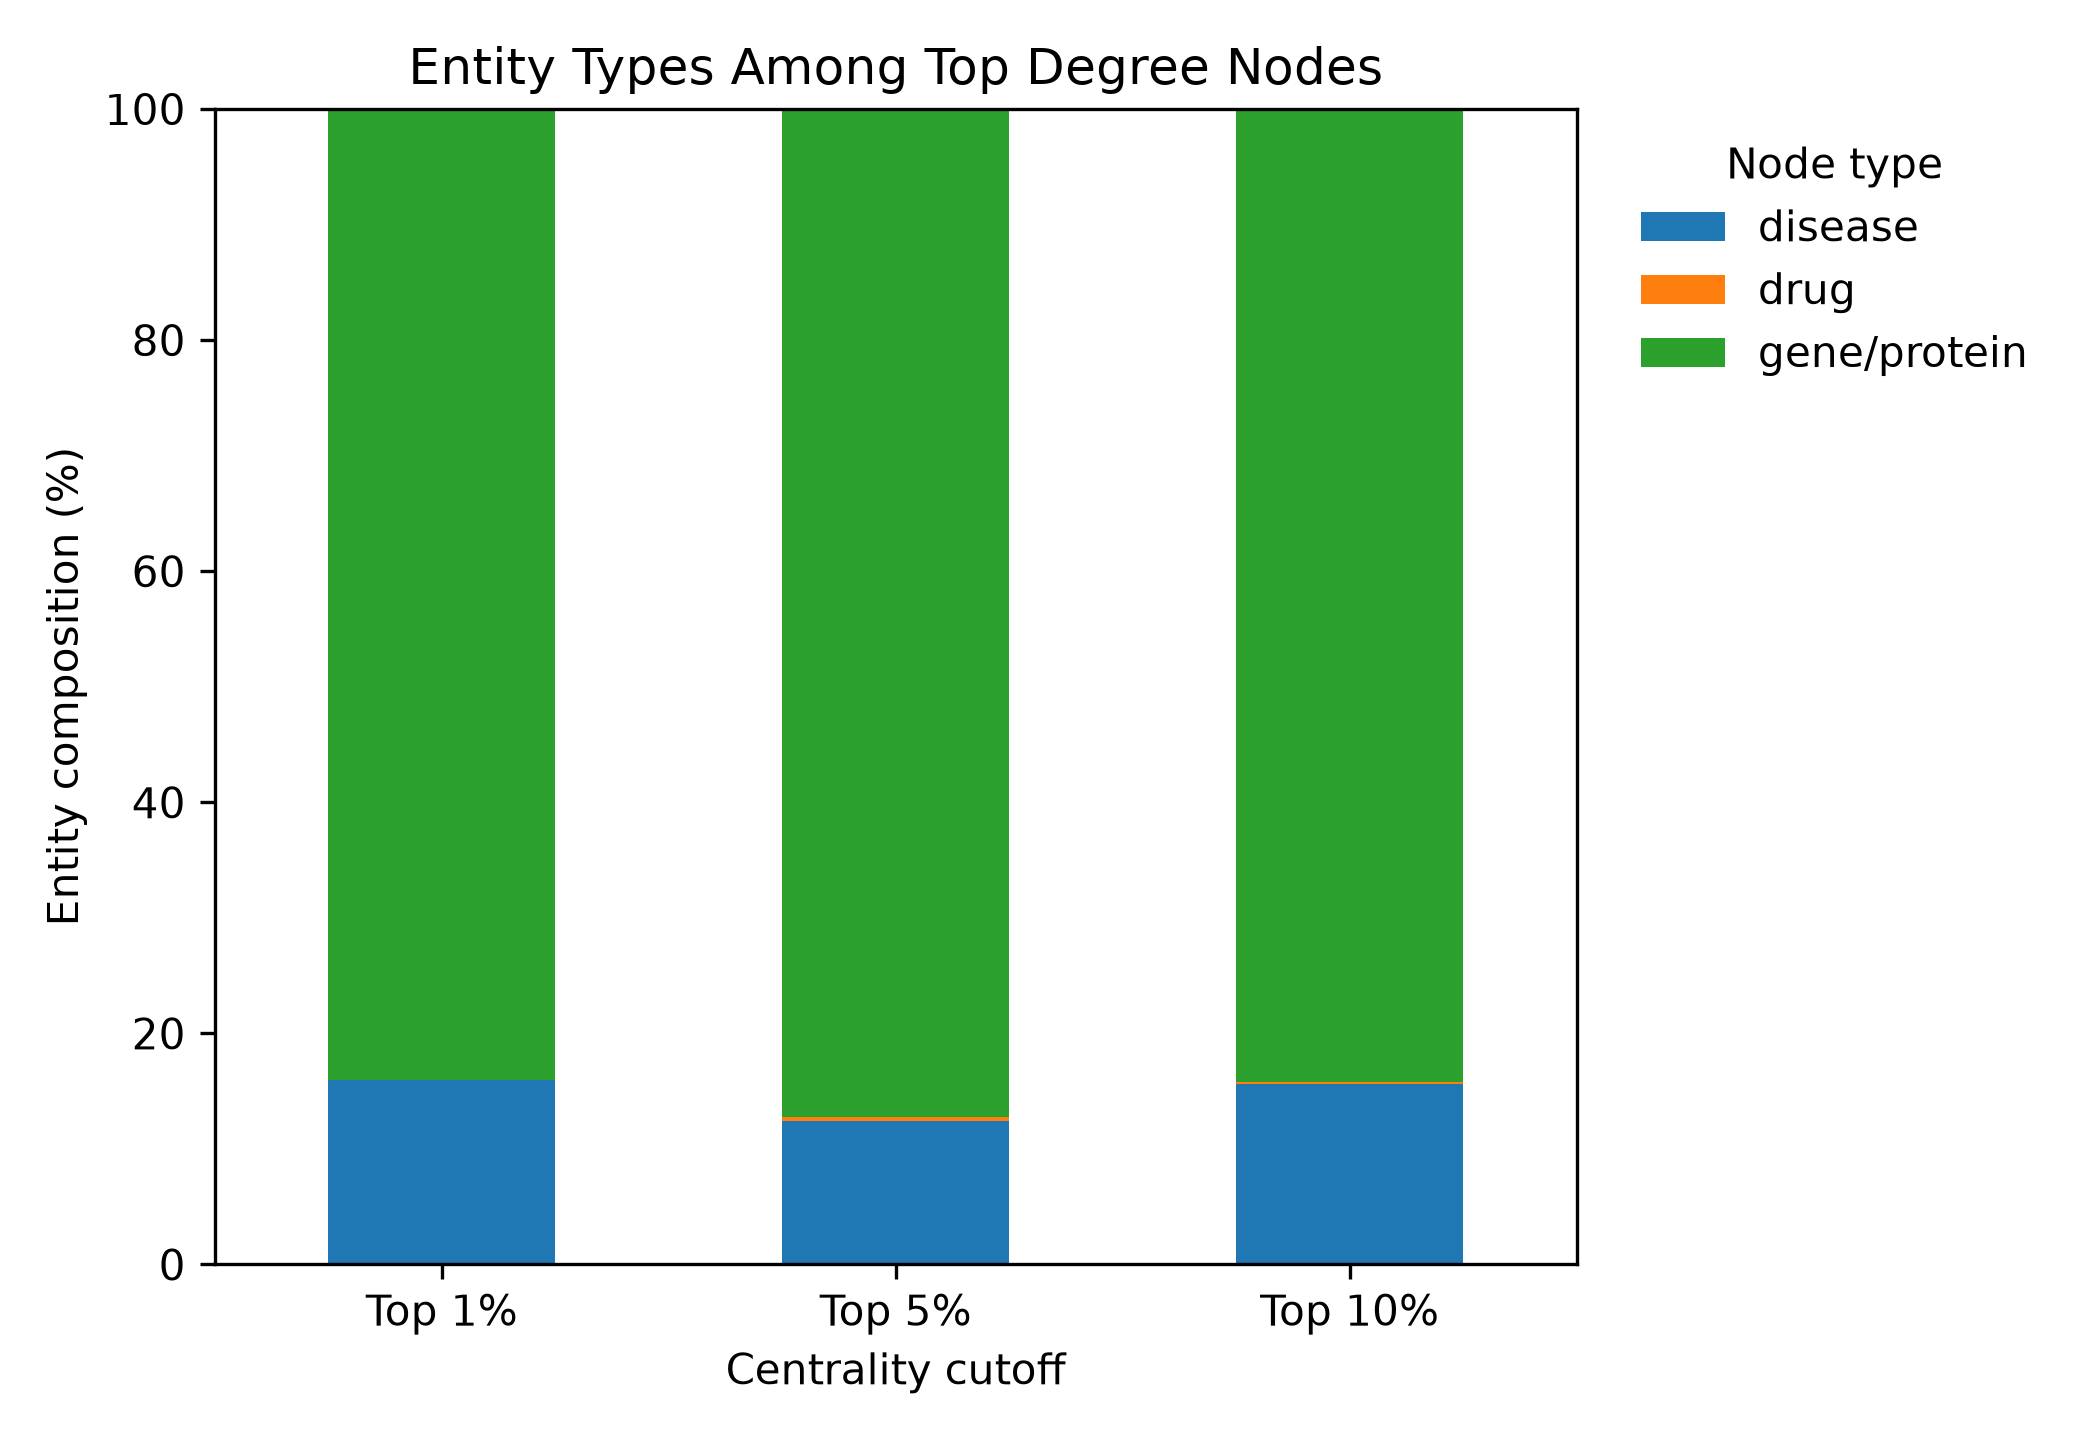
\includegraphics[width=\linewidth]{ws2_degree_hub_composition_primekg_5000_bfs_v1.png}
      \caption{Degree ranking}
      \end{subfigure}\hfill
      \begin{subfigure}{0.48\linewidth}
      \centering
      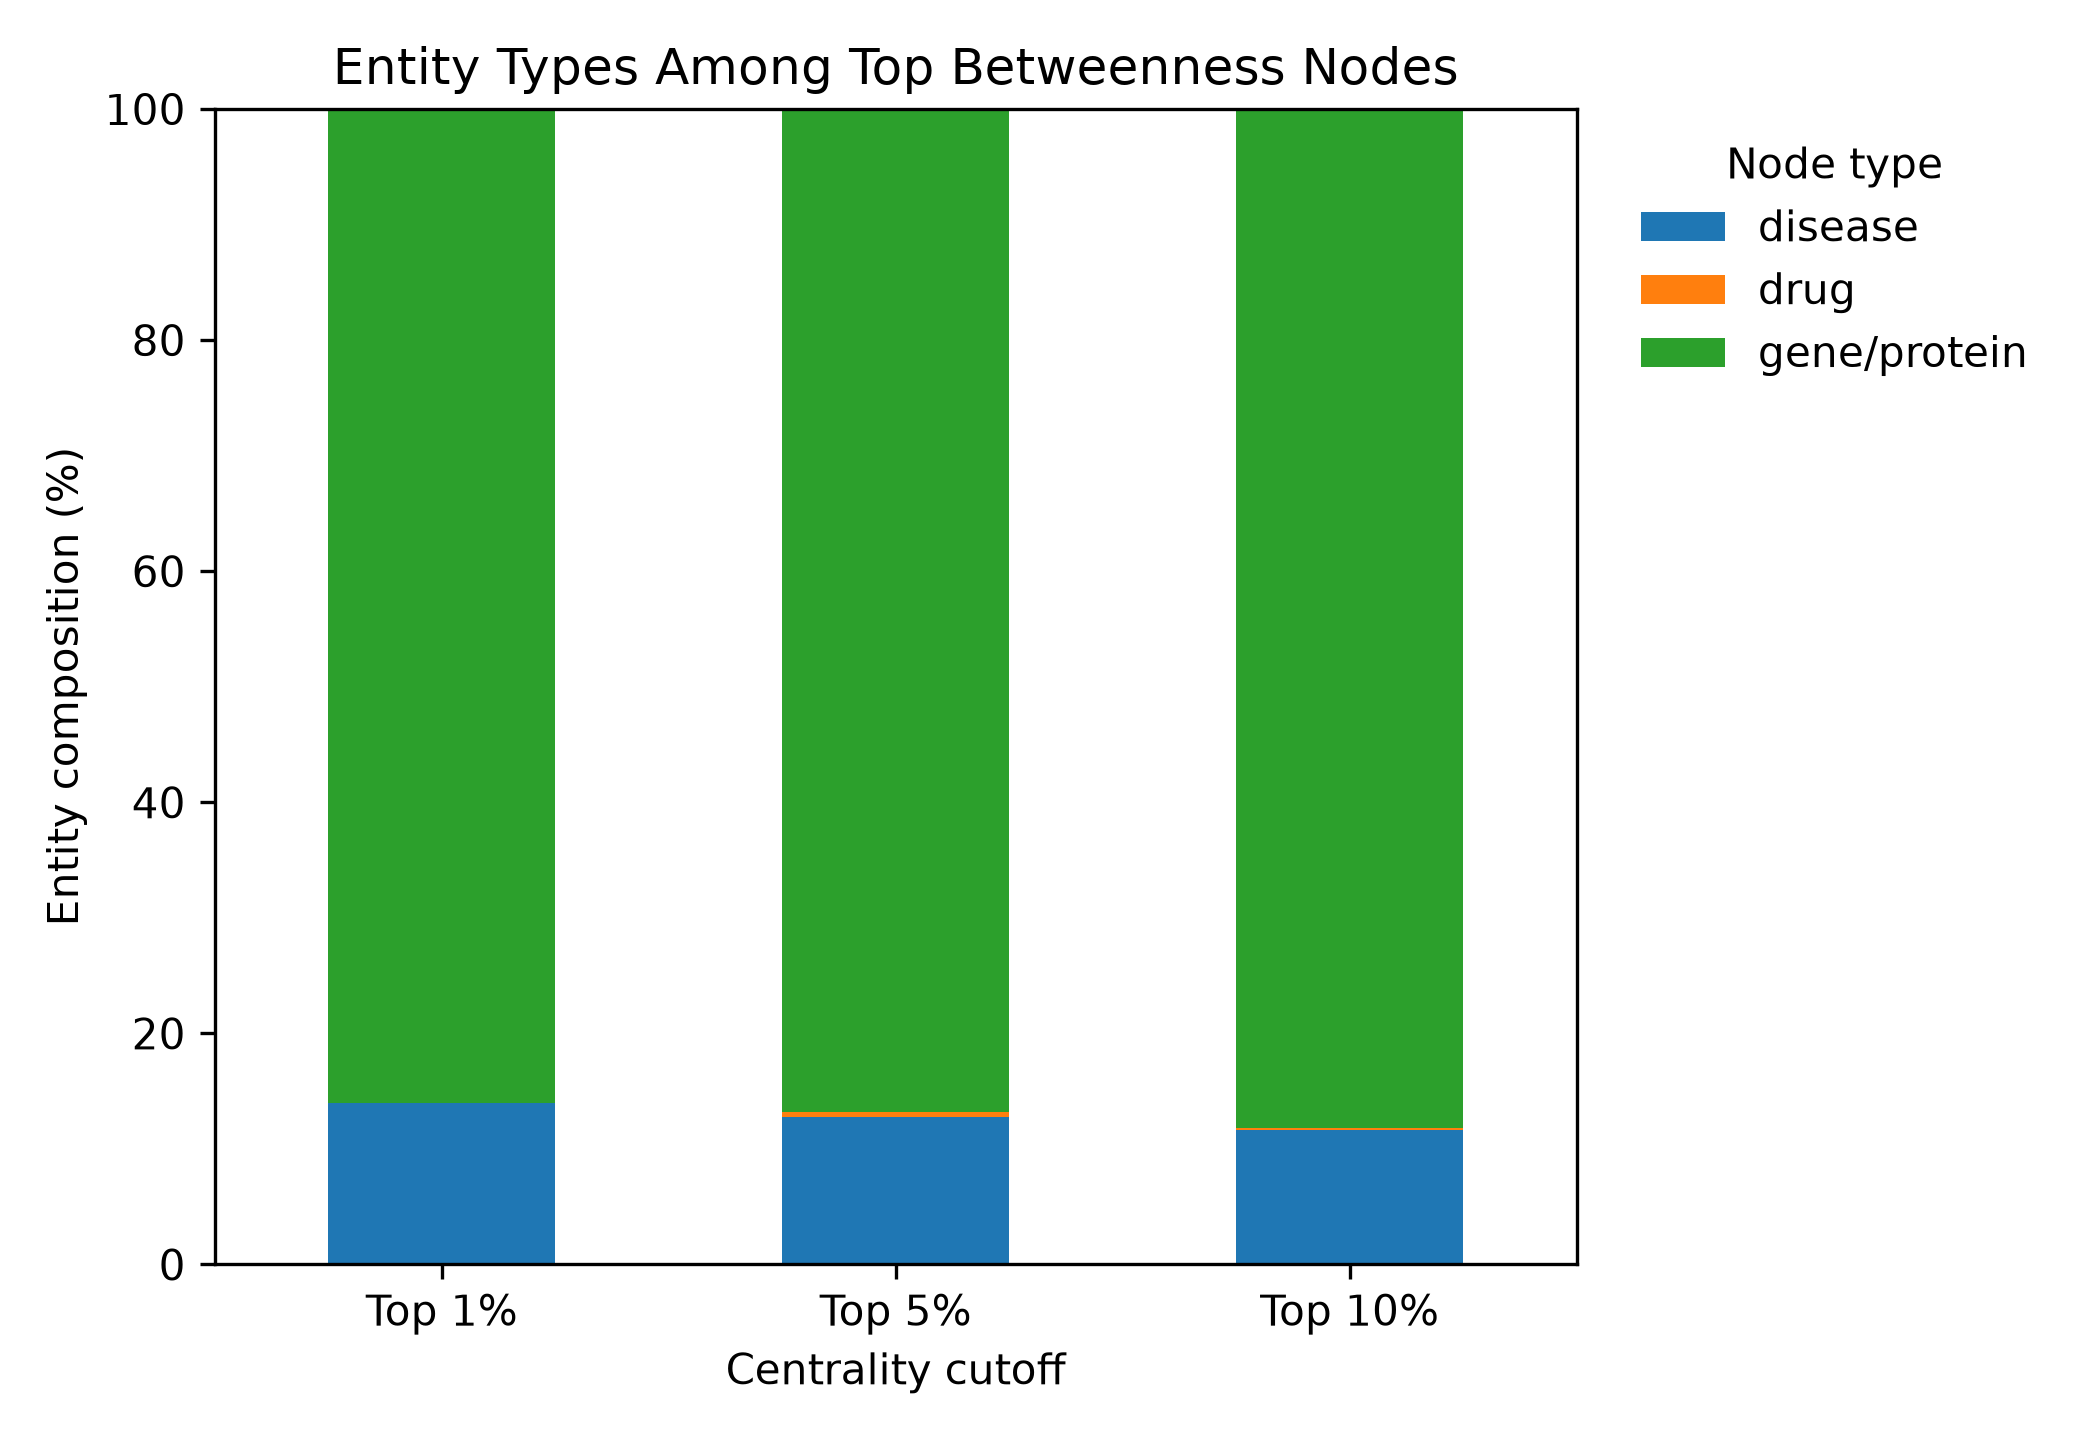
\includegraphics[width=\linewidth]{ws2_betweenness_hub_composition_primekg_5000_bfs_v1.png}
      \caption{Betweenness ranking}
      \end{subfigure}%
      }{%
      \fbox{\parbox[c][2.0in][c]{0.82\linewidth}{\centering Placeholder: central-node entity composition figures}}%
      }%
    }
    \caption{Entity-type composition among highly central nodes. Disease nodes constitute 5.66\% of the full graph but 14--16\% of the top 1\% central nodes.}
    \label{fig:ws2-composition}
\end{figure}

The two rankings also show substantial agreement at the individual-node level. Let $D_{50}$ and $B_{50}$ denote the top 50 nodes under degree and betweenness. Their intersection contains 41 nodes, and their Jaccard similarity is
\begin{equation}
J(D_{50},B_{50})=\frac{|D_{50}\cap B_{50}|}{|D_{50}\cup B_{50}|}=\frac{41}{59}\approx0.695.
\end{equation}
This strong overlap helps explain why the degree- and betweenness-based attack curves are similar: many nodes removed early under one ranking are also removed early under the other. The disease enrichment should be interpreted as a structural observation about this graph construction rather than as a direct biomedical claim.

\subsubsection{Comparison with the Theoretical Reference}
The final presentation also compares the empirical degree attack with the degree-based theoretical reference developed in Section~\ref{sec:theory}. The theoretical curve captures the broad collapse pattern but does not perfectly reproduce the empirical trajectory. This suggests that degree information alone does not capture every structural feature that influences the response of the empirical PrimeKG subgraph to targeted removal. The theoretical derivation and a systematic analysis of this discrepancy are left to the theory and prediction sections; here the comparison provides an empirical bridge between targeted robustness and the project's null-model analysis.

Overall, the targeted-attack experiments show that the identity of failed nodes matters strongly for structural robustness. Random node loss leaves a substantially larger connected core than removal of high-centrality nodes, while degree and betweenness identify a strongly overlapping critical set. The next section moves from structural robustness to functional robustness and asks whether drug--disease queries remain answerable after graph damage.


\section{Functional Robustness and Query Horizon}
\label{sec:functional}

\subsection{Retrieval under controlled damage}
\label{retrieval-under-controlled-damage}

We evaluated retrieval on the 5,000-node PrimeKG subgraph using the fixed
benchmark from Section~\ref{sec:data}. The benchmark contains 200
drug--disease pairs that were retrievable in two hops before damage. One hundred had one such path, and one hundred had multiple paths. We used the same
queries and group assignments at every damage level. If a drug or
disease was removed, its query counted as a failure and remained in
the denominator.

For each damaged graph, the retriever builds sets of the surviving
protein neighbors of each drug and disease. A two-hop query succeeds
when those sets intersect. The size of the intersection is the number
of surviving two-hop paths. For larger hop limits, the retriever
computes the shortest unweighted distance $d_{\mathrm{PPI}}$ between
the two neighbor sets along surviving protein--protein interaction
(PPI) edges. A shared protein gives $d_{\mathrm{PPI}}=0$. If either set
is empty or no connecting PPI path exists, the distance is infinite.
The shortest allowed drug--disease path therefore has length
$2+d_{\mathrm{PPI}}$, including one edge at each endpoint. For a
finite hop limit $L$, a query succeeds when this length is at most
$L$. For unlimited hops, a query succeeds when the distance is finite.
We write $R_L(f)$ for the fraction of benchmark queries that succeed
at removal fraction $f$ and hop limit $L$.

The two-hop experiments used ten seeds (0--9) for each random removal
strategy and one fixed order each for degree- and betweenness-targeted
node removal. The hop scan used random edge removal with the same
three seeds (0--2) for $L=2,3,4,\infty$. Matching the queries and the
damage states across hop limits isolates the effect of changing $L$.

\subsection{Connectivity and retrieval under damage}
\label{connectivity-and-retrieval-separate}

At 50\% random edge removal, the largest connected component still
contained 98.2\% of the original nodes, whereas two-hop retrieval
succeeded for 43.3\% of the benchmark queries. The gap was 54.9
percentage points across the same ten damage seeds
(Figure~\ref{fig:ws3-structure-vs-retrieval}). Protein--protein edges
can keep much of the graph connected even after a query has lost its
last shared-protein route. The largest-component fraction $S(f)$ can
therefore remain high while $R_2(f)$ declines.

\begin{figure}[!htbp]
  \centering
  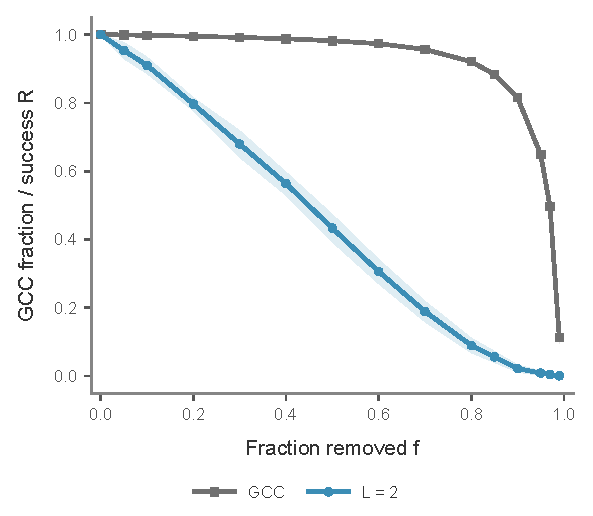
\includegraphics[width=0.88\linewidth]{act2/primekg_5000_bfs_v1/fig_S_vs_R.pdf}
  \caption{Largest connected component fraction $S(f)$ and two-hop retrieval success $R(f)$ under random edge removal. Curves are means across ten seeds. Shading shows one sample standard deviation on either side of the mean.}
  \label{fig:ws3-structure-vs-retrieval}
\end{figure}

Deleting nodes removes their incident edges and can also remove the
query endpoints themselves. At 50\% node removal, mean two-hop success
was 15.55\% under random deletion. It fell to 0\% under the fixed
degree ranking and 0.5\% under the fixed betweenness ranking. These
two targeted results describe individual deletion orders.

\subsection{Path redundancy and two-hop survival}
\label{backup-paths-and-hop-limits}

At 50\% random edge removal, two-hop success was 60.7\% for queries
with multiple original paths and 25.9\% for queries with one original
path (Figure~\ref{fig:ws3-path-redundancy}). The groups are defined by
their intact-graph path counts. A query with multiple paths remains
retrievable as long as both edges of any one of its original
shared-protein routes survive.

Under independent edge retention with probability $p$, each two-hop
path survives with probability $p^2$. Routes through distinct shared
proteins use distinct edges, so a query with $m$ such routes has
survival probability $1-(1-p^2)^m$. We used this model as a benchmark
for the fixed-count deletion experiments, averaging the predicted
probabilities over the queries in each group. On the 5,000-node graph,
the largest absolute differences between observed and predicted
group means across the tested fractions were 2.10 percentage points for
single-path queries and 3.25 for multi-path queries. The single-path
group on the 2,000-node development graph showed a larger maximum
deviation of 9.05 percentage points. The retriever agreed with an
independent NetworkX implementation on the checked development cases.

\begin{figure}[!htbp]
  \centering
  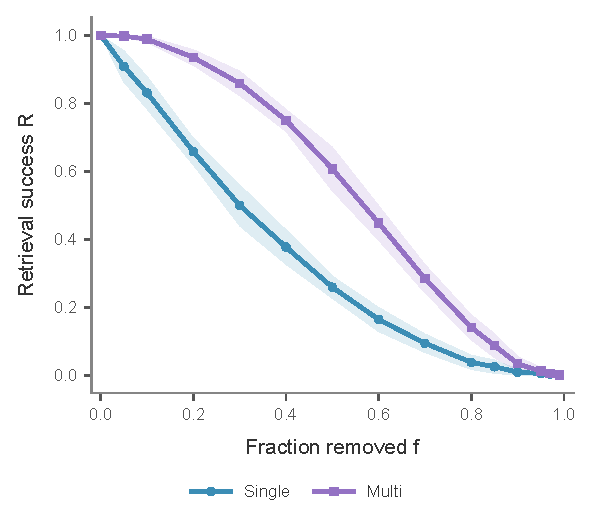
\includegraphics[width=0.88\linewidth]{act2/primekg_5000_bfs_v1/fig_R_by_group.pdf}
  \caption{Two-hop retrieval success under random edge removal, grouped by whether a query had one or multiple two-hop paths before damage. Curves are means across ten seeds. Shading shows one sample standard deviation on either side of the mean.}
  \label{fig:ws3-path-redundancy}
\end{figure}

\subsection{Effect of the hop limit}

In the matched three-seed comparison, allowing one additional PPI
step at 50\% edge removal increased mean retrieval success from
40.3\% at $L=2$ to 84.5\% at $L=3$. The mean reached 89.5\% at $L=4$
and stayed at 89.5\% with unlimited hops. The two-hop value here is
the baseline for the three scan seeds. The 43.3\% reported above is
the mean over all ten seeds.

At 90\% edge removal, the corresponding success rates were 2.0\%,
10.0\%, 28.7\%, and 37.0\%. At this higher damage level, the
8.3-percentage-point gap between four hops and unlimited hops shows
that some surviving routes require more than two PPI steps.
Figures~\ref{fig:ws3-hop-curves} and~\ref{fig:ws3-hop-heatmap} show how
success varies with the removal fraction and the hop limit. The
results describe typed path availability for an initially retrievable,
redundancy-balanced benchmark on a BFS-sampled subgraph. The measured
rates depend on both the benchmark and the allowed path length.

\begin{figure}[!htbp]
  \centering
  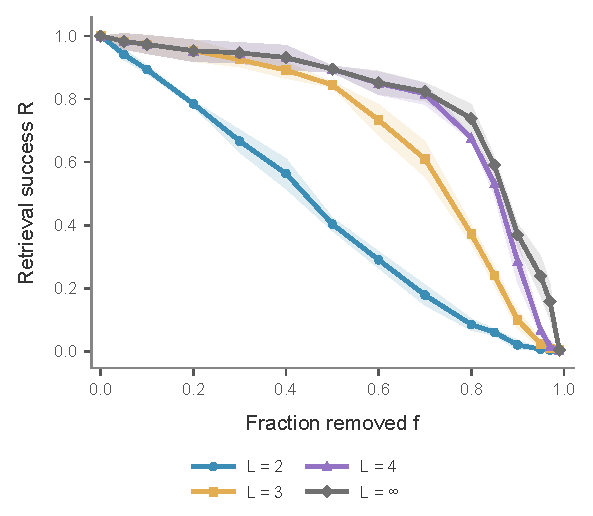
\includegraphics[width=0.88\linewidth]{act2/primekg_5000_bfs_v1/fig_R_L_curves.pdf}
  \caption{Retrieval success under random edge removal for hop limits $L=2,3,4,\infty$. All curves use the same three removal seeds. Shading shows one sample standard deviation on either side of the mean.}
  \label{fig:ws3-hop-curves}
\end{figure}

\begin{figure}[!htbp]
  \centering
  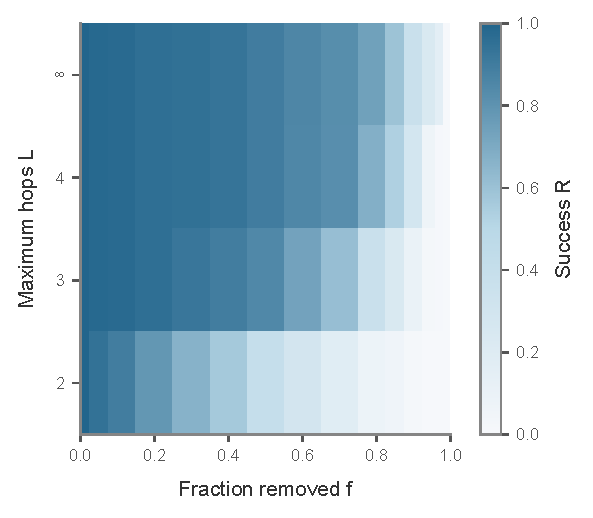
\includegraphics[width=0.88\linewidth]{act2/primekg_5000_bfs_v1/fig_R_L_heatmap.pdf}
  \caption{Mean retrieval success by edge removal fraction $f$ and hop limit $L$. Each cell averages the same three random edge removal seeds used in Figure~\ref{fig:ws3-hop-curves}.}
  \label{fig:ws3-hop-heatmap}
\end{figure}

We ran the retrieval experiments with \texttt{src/run\_ws3.py},
saved the results in \texttt{results/ws3}, and generated the four
figures with \texttt{src/plot\_ws3.py}.

\section{Predicting Retrieval Failure}
\label{sec:prediction}
% Owner: D. Target: about 1 page.
\textit{[D: connect the theoretical model to retrieval-failure prediction here.]}

\section{Network-Informed Restoration}
\label{sec:restoration}

\subsection{Shared damage states and repair budgets}
\label{shared-damage-states-and-repair-budgets}

On the 5,000-node graph, we randomly removed 30\% or 50\% of the edges
(35,367 or 58,946 edges) while keeping all nodes intact. For each deletion
fraction $f$ and each of ten random damage orders, all four policies started
from the same damaged graph and restored 0\%, 5\%, 10\%, or 20\% of the
deleted edges. At the 5\%, 10\%, and 20\% budgets, policies restored 1,768,
3,537, and 7,073 edges after 30\% deletion, and 2,947, 5,895, and 11,789
edges after 50\% deletion, with every policy filling its budget in full.

The 200 queries were split by query ID into 140 training queries for
edge ranking and 60 held-out test queries for evaluation, ensuring that
test queries never informed policy rankings. After each repair, we measured
the giant connected component (GCC) as a fraction of the original 5,000
nodes alongside held-out retrieval success at $L=2$ and $L=3$. Before
repair, the unrepaired baselines already differed sharply across metrics:
at $f=0.30$, mean unrepaired values were $99.204 \pm 0.104\%$ for GCC,
$93.50 \pm 5.18\%$ for $L=3$, and $68.33 \pm 6.38\%$ for $L=2$; at
$f=0.50$, they were $98.218 \pm 0.128\%$ for GCC, $83.50 \pm 7.13\%$ for
$L=3$, and $42.33 \pm 4.32\%$ for $L=2$. Subtracting each seed's unrepaired
baseline from its post-repair value gives paired gains, which we summarize
as means and sample standard deviations (SD) across the ten seeds.

\subsection{Four restoration policies}
\label{four-restoration-policies}

Each policy defines a fixed ordering over deleted edges on a given damaged
graph, so larger budgets restore longer prefixes of the same ranking.
Random restoration shuffles all deleted edges uniformly and serves as an
uninformed baseline. Edge-betweenness restoration filters the intact-graph
edge-betweenness ranking to the deleted edges, prioritizing structural
bridges without using query or relation labels. Relation-type restoration
randomly orders deleted drug--protein and disease--protein edges without
substituting protein--protein interactions, isolating the effect of
restricting repairs to the relation types required by two-hop paths.

Static task-aware restoration scores deleted edges once on the initial
damaged graph using training queries that have lost all two-hop paths. Each
broken two-hop path missing exactly one edge contributes one point to that
missing edge, while paths missing both edges and already-successful
training queries contribute zero. Deleted edges are then ranked in
descending order of score, with ties---including zero-score edges---broken
randomly.

\subsection{Recovery depends on target metric, budget, and query horizon}
\label{recovery-depends-on-budget-and-query-horizon}

Figure~\ref{fig:restoration-retrieval} compares held-out retrieval gains
across both damage levels and query horizons, and
Table~\ref{tab:restoration-gains} summarizes the 20\% budget at $f=0.50$.
Across these settings, policy performance depends strongly on whether
repair targets global connectivity, short-horizon retrieval ($L=2$), or
longer-horizon retrieval ($L=3$).

\begin{table}[htbp]
  \centering
  \caption{Paired gains after restoring 20\% of the edges removed at
  $f=0.50$ (11,789 restored edges). Values are means $\pm$ sample SD in
  percentage points over ten damage seeds. Unrepaired baselines are
  $42.33 \pm 4.32\%$ ($L=2$), $83.50 \pm 7.13\%$ ($L=3$), and
  $98.218 \pm 0.128\%$ (GCC).}
  \label{tab:restoration-gains}
  \begin{tabular}{@{}lccc@{}}
    \toprule
    Policy & $L=2$ retrieval & $L=3$ retrieval & GCC fraction \\
    \midrule
    Random            & $13.17 \pm 2.77$ & $8.33 \pm 5.77$  & $0.584 \pm 0.106$ \\
    Edge betweenness  & $42.00 \pm 3.99$ & $16.50 \pm 7.13$ & $1.782 \pm 0.128$ \\
    Relation type     & $48.50 \pm 6.69$ & $15.67 \pm 7.34$ & $0.610 \pm 0.129$ \\
    Static task-aware & $24.83 \pm 6.31$ & $12.33 \pm 6.63$ & $0.670 \pm 0.085$ \\
    \bottomrule
  \end{tabular}
\end{table}

\begin{figure}[htbp]
  \centering
  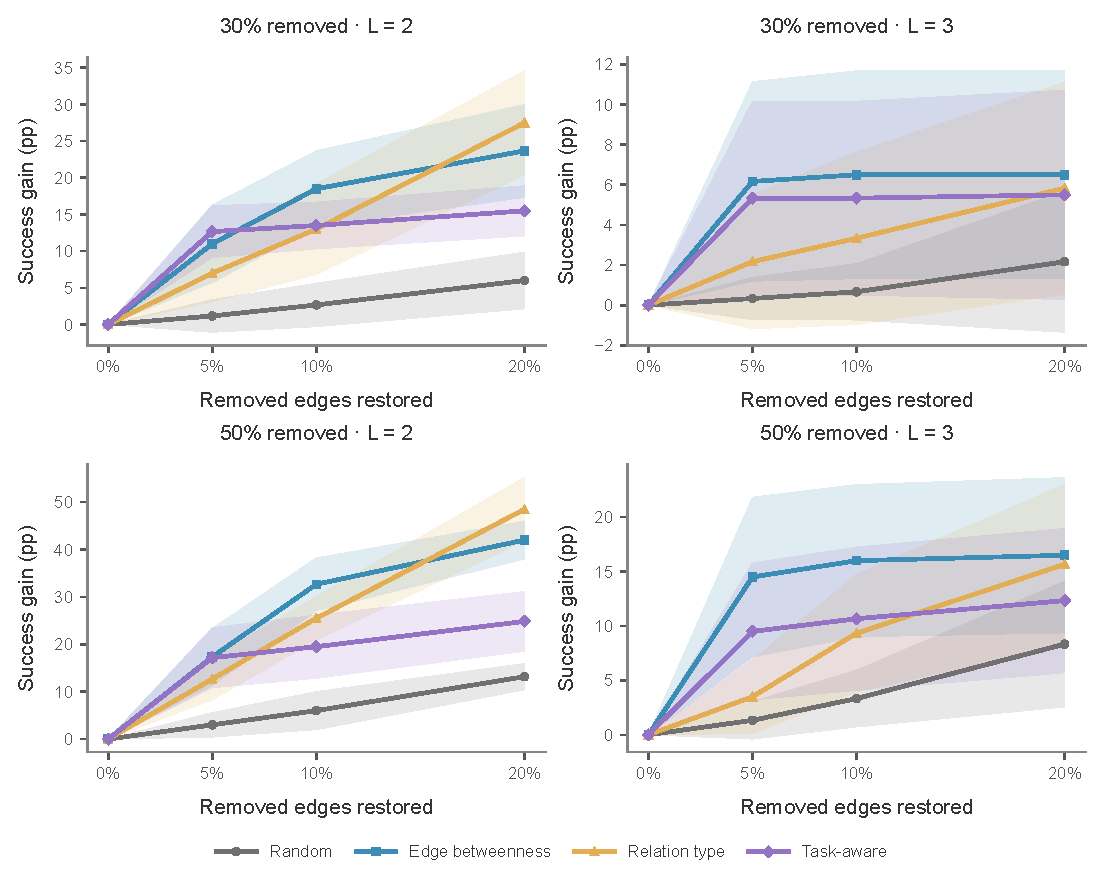
\includegraphics[width=\linewidth]{act3/final/primekg_5000_bfs_v1/fig_restoration.pdf}
  \caption{Held-out retrieval gains for the four repair policies at $L=2$ and
  $L=3$, after 30\% or 50\% edge loss. The horizontal axis gives the share of
  deleted edges restored. Lines show means of paired gains over ten damage
  seeds, and shading shows one sample SD.}
  \label{fig:restoration-retrieval}
\end{figure}

For two-hop retrieval, policy rankings cross over as the budget grows. At
30\% edge loss and a 5\% budget (1,768 edges), static task-aware repair
achieved the largest mean two-hop gain at $12.67 \pm 3.53$ percentage
points, ahead of edge betweenness ($11.00 \pm 5.28$), relation type
($7.00 \pm 3.91$), and random ($1.17 \pm 2.23$). At 50\% edge loss and a
5\% budget (2,947 edges), edge betweenness ($17.33 \pm 5.99$) and static
task-aware ($17.17 \pm 6.34$) were nearly tied at the top, ahead of
relation type ($12.67 \pm 4.39$) and random ($3.00 \pm 2.58$). Once the
budget reached 20\%, however, relation type pulled clearly ahead at both
damage levels, gaining $27.50 \pm 7.08$ points at $f=0.30$ and
$48.50 \pm 6.69$ points at $f=0.50$ (recovering 84\% of the lost two-hop
queries), compared with $23.67$ and $42.00$ points for edge betweenness and
only $15.50$ and $24.83$ points for static task-aware.

Marginal efficiency, plotted in Figure~\ref{fig:restoration-efficiency} as
paired retrieval gain per 1,000 restored edges, highlights the same
contrast between front-loaded and steady policies. At $f=0.30$ and a 5\%
budget, static task-aware delivered the highest efficiency at $7.16$
percentage points per 1,000 edges (versus $6.22$ for edge betweenness and
$3.96$ for relation type), but its efficiency fell steeply to $2.19$ points
per 1,000 edges at the 20\% budget ($5.83 \to 2.11$ at $f=0.50$).
Relation-type repair, in contrast, maintained nearly flat marginal returns
across all budgets ($3.96 \to 3.68 \to 3.89$ at $f=0.30$;
$4.30 \to 4.33 \to 4.11$ at $f=0.50$).

\begin{figure}[htbp]
  \centering
  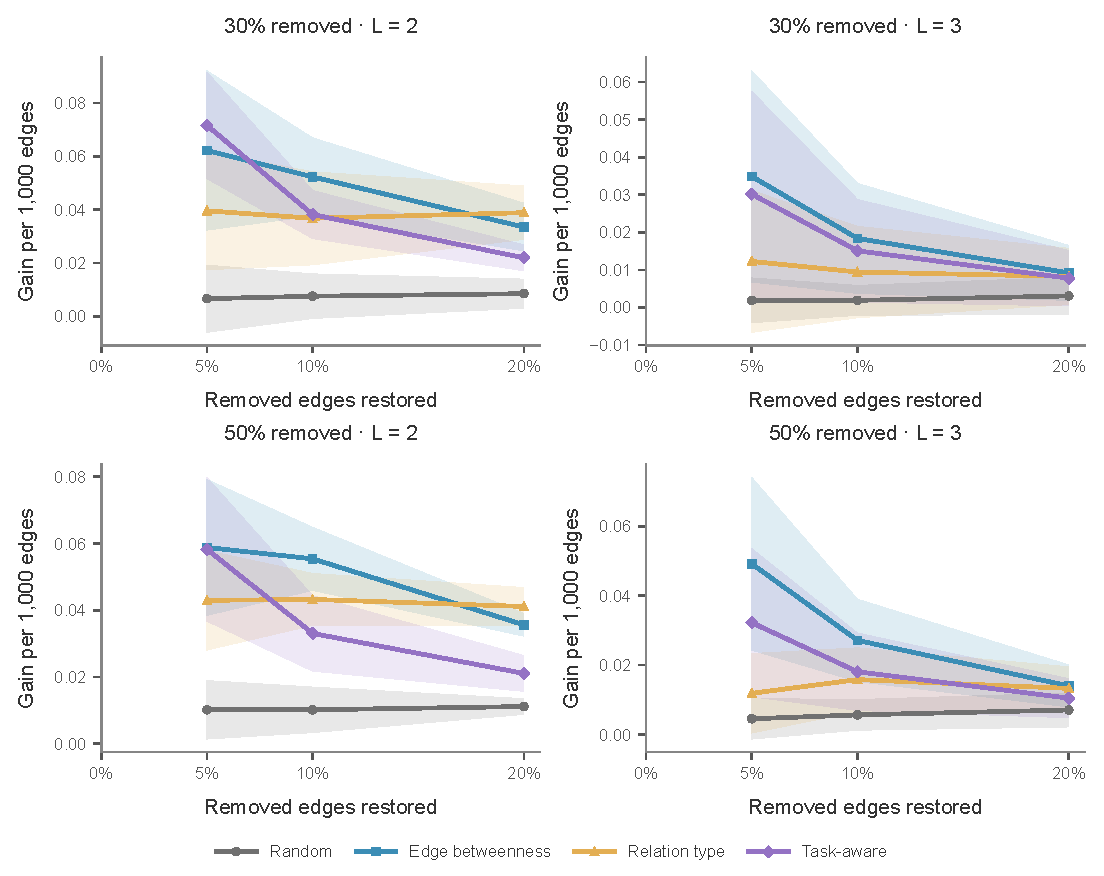
\includegraphics[width=\linewidth]{act3/final/primekg_5000_bfs_v1/fig_gain_per_edge.pdf}
  \caption{Mean gain in retrieval success fraction per 1,000 restored edges.
  For each seed, we divide the paired gain by the actual number of restored
  edges and multiply by 1,000 before averaging. Shading shows one sample SD
  across ten seeds. Efficiency is defined only for positive repair budgets.}
  \label{fig:restoration-efficiency}
\end{figure}

Global connectivity and longer-horizon retrieval instead favored edge
betweenness and reached their ceilings early. At 50\% edge loss, edge
betweenness increased the GCC fraction by $1.782 \pm 0.128$ points already
at the 10\% budget---completely restoring 100\% GCC connectivity---whereas
random ($0.584$), relation type ($0.610$), and static task-aware ($0.670$)
remained below $0.7$ points even at the 20\% budget
(Table~\ref{tab:restoration-gains} and Figure~\ref{fig:restoration-gcc}).
The same full GCC recovery occurred by the 10\% budget at $f=0.30$
($+0.796$ points). At $L=3$, the unrepaired baseline is already high
($93.50\%$ at $f=0.30$ and $83.50\%$ at $f=0.50$), leaving less headroom.
Edge betweenness closed the entire $L=3$ gap ($+6.50$ points by the 10\%
budget at $f=0.30$; $+16.50$ points at the 20\% budget at $f=0.50$), while
relation type reached $+15.67$ points at $f=0.50$, leaving only a narrow
$0.83$-point margin right against the 100\% ceiling. Thus, the policy that
maximized structural recovery differed from the policy that maximized
large-budget two-hop retrieval.

\begin{figure}[htbp]
  \centering
  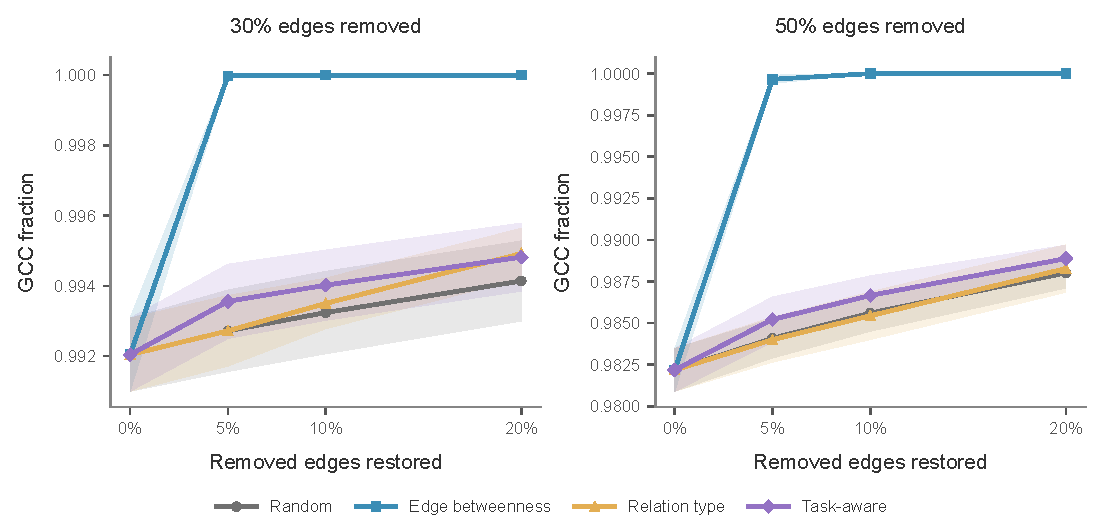
\includegraphics[width=\linewidth]{act3/final/primekg_5000_bfs_v1/fig_restoration_gcc.pdf}
  \caption{GCC fraction after repair at 30\% and 50\% initial edge loss.
  Values are fractions of the original 5,000 nodes. Lines show means and
  shading shows one sample SD over the ten damage seeds.}
  \label{fig:restoration-gcc}
\end{figure}

\subsection{Why the policies diverge: score saturation and edge-type mix}
\label{interpreting-the-static-score}

Two diagnostics explain both the budget crossover and the gap between
structural and functional recovery. First, the static task-aware score
saturates almost immediately. Across the ten damage seeds, only 31--46
deleted edges had positive static scores at 30\% deletion and 62--87 at 50\%
deletion. Those edges accounted for at most $2.6\%$ (at $f=0.30$) and
$3.0\%$ (at $f=0.50$) of the 5\% budget, and less than $0.8\%$ of the 20\%
budget. After restoring that small set of high-impact edges---which drives
its strong 5\%-budget jump---the policy spends more than 97\% of the budget
on randomly ordered zero-score edges, effectively behaving like random
repair thereafter.

Second, Figure~\ref{fig:restoration-composition} shows how each policy
allocated its budget across relation types. In the intact 5,000-node graph,
protein--protein interactions make up 76.5\% of all edges, disease--protein
relations 23.1\%, and drug--protein relations only 0.40\%. At 50\% edge loss
and a 20\% budget, static task-aware repair spent 76.0\% of its budget on
protein--protein edges (matching random's 76.4\% once zero-score ties
dominate), and edge betweenness spent 68.1\% on protein--protein edges.
Relation-type repair instead spent 100\% of its budget on the terminal
relations required by two-hop paths (98.3\% disease--protein and 1.7\%
drug--protein), explaining its sustained $L=2$ gains at larger budgets.

\begin{figure}[H]
  \centering
  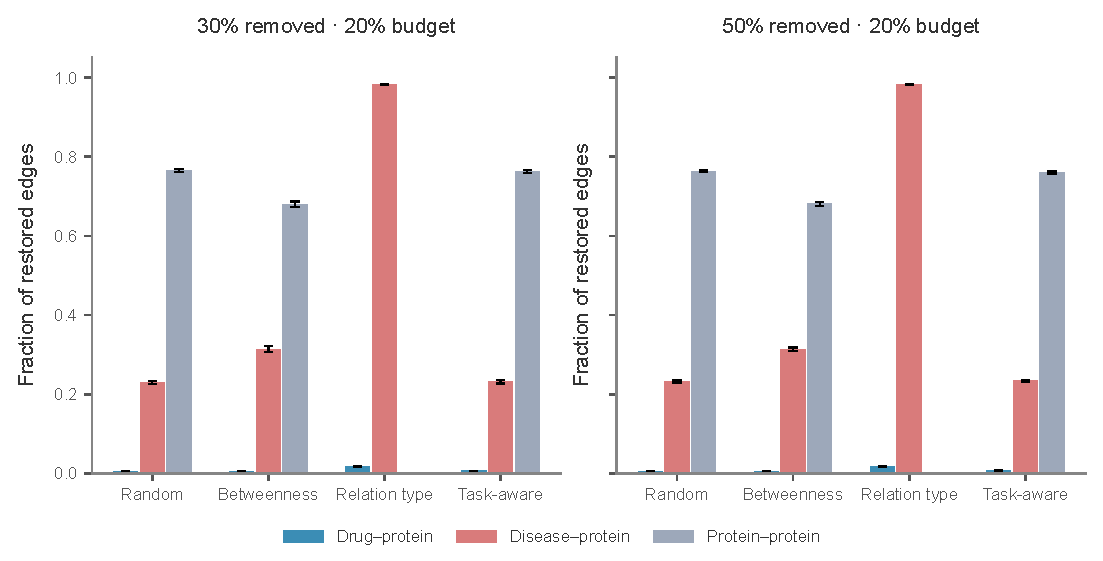
\includegraphics[width=0.9\linewidth]{act3/final/primekg_5000_bfs_v1/fig_restored_edge_types.pdf}
  \caption{Relation types among the edges actually restored with a 20\% repair
  budget. Bars show the mean share of each relation type. Error bars show one
  sample SD over ten damage seeds.}
  \label{fig:restoration-composition}
\end{figure}

Edge-type allocation also clarifies why edge betweenness performed much
better on $L=2$ than random repair despite ignoring relation labels. Because
drugs have much lower mean degree than proteins or diseases
(Section~\ref{sec:data}), deleted drug--protein edges often act as
high-betweenness bridges: at the 5\% budget, drug--protein edges made up
$1.31$--$1.34\%$ of edge-betweenness repairs, more than three times their
$0.42$--$0.44\%$ share under random repair. At the same time, its large
allocation to high-betweenness protein--protein bridges explains why it
dominated GCC and $L=3$ recovery, where a single protein--protein step can
reconnect many failed queries.

These results also point to clear directions for refinement. Because the
140/60 split is defined over query IDs, training and test queries can share
drug or disease endpoints, and the static score is computed once from
two-hop training paths without updating as edges are restored or adapting
to three-hop paths. Extending the scoring rule to update iteratively or to
incorporate longer paths would test how much further task-aware restoration
can go once score saturation is removed.

\section{Discussion, Limitations, and Conclusion}
\label{sec:discussion}

\subsection{Discussion}
Our results show that network robustness depends on what we want the network to preserve. Random edge removal left a large connected core in the 5,000-node BFS graph: at $f=0.50$, the largest connected component still contained 98.2\% of the original nodes, close to the configuration-model reference. However, only 43.3\% of the fixed queries retained a valid two-hop path on the same ten damage states (Section~\ref{sec:functional}). Protein--protein interactions can preserve global connectivity even when a drug and disease lose their last shared-protein route. Thus, connectivity alone is not a sufficient measure of functional robustness.

The type and location of damage also matter. In Section~\ref{sec:structural}, targeted removal of high-degree or high-betweenness nodes reduced the giant component more rapidly than random node removal. At $f=0.50$, the remaining giant-component fractions were approximately 0.232 and 0.206 under these fixed targeted rankings, versus 0.493 under random removal. The two centrality rankings overlapped substantially, but the observed patterns apply to the fixed rankings used here rather than adaptive attacks.

Functional performance also depends on the permitted query horizon. At 50\% random edge removal, the matched three-seed comparison increased retrieval success from 40.3\% at $L=2$ to 84.5\% at $L=3$. Queries with multiple original shared-protein paths were more likely to retain a two-hop route than single-path queries (60.7\% versus 25.9\% at the same damage level). Both path redundancy and allowing additional hops can therefore buffer query failure, although they describe different mechanisms.

Restoration results extend this distinction from robustness to recovery. No single policy performed best for all targets and budgets (Section~7). Edge-betweenness repair quickly restored global connectivity and three-hop reachability; relation-type repair achieved the largest two-hop gain at a 20\% budget after 50\% edge removal (48.50 percentage points). Static task-aware repair was competitive at the smallest budget, but its fixed scores quickly saturated, leaving most of the remaining budget to zero-score ties. These differences show why repair priorities should follow the intended retrieval task and available budget rather than topology alone.

% TODO(D): Integrate D's validated theory and retrieval-failure prediction findings here once supplied.

\subsection{Limitations}
The standard 5,000-node graph is a deterministic BFS sample, not a representative random sample of the filtered PrimeKG network. At 90\% random edge removal, its giant-component fraction was 81.5\%, compared with 55.4\% for the filtered full graph. This comparison shows a substantial sampling sensitivity, but does not isolate the individual effects of graph size, composition, and degree distribution.

Our functional benchmark consists of 200 initially retrievable drug--disease pairs, balanced between single-path and multi-path cases. It therefore measures survival under a controlled task distribution, not the prevalence of retrievable relations among arbitrary pairs. The hop-limit scan uses only three random edge-removal seeds, while several other comparisons use ten; results should be interpreted with their stated seed counts. A surviving typed association path also does not establish a clinically meaningful treatment relationship.

The targeted attacks use centrality rankings computed on the intact graph, without recomputation after removal. The retrieval model tests path availability under specified relation and hop constraints rather than a complete biomedical reasoning system. Restoration is evaluated on the BFS subgraph, and the task-aware policy uses a one-time two-hop score based on training paths missing one edge; it does not update scores during repair or consider paths missing both edges. The 140/60 training/test split separates query IDs, not entities, so endpoints may overlap across splits. These choices support controlled comparisons but limit generalization.

% TODO(D): Add any specific limitations of D's theoretical approximation and prediction model once verified.

\subsection{Conclusion}
A knowledge graph can remain largely connected while losing many of the short, typed paths needed by its queries. Our PrimeKG experiments show that structural robustness, functional retrieval, and recovery under repair budgets are related but distinct outcomes. Redundant paths and longer query horizons improve retrieval survival, while the most effective repair strategy changes with the objective and budget. A practical robustness assessment should therefore report both network connectivity and task-specific retrieval success, with explicit graph, query, and damage definitions.

% TODO(D): Revisit the final synthesis after Sections 3 and 6 are completed.


\clearpage
\begin{thebibliography}{9}
\bibitem{chandak2023primekg} P. Chandak, K. Huang, and M. Zitnik, ``Building a knowledge graph to enable precision medicine,'' \textit{Scientific Data}, vol. 10, 67, 2023.
\bibitem{albert2000error} R. Albert, H. Jeong, and A.-L. Barabasi, ``Error and attack tolerance of complex networks,'' \textit{Nature}, vol. 406, pp. 378--382, 2000.
\bibitem{newman2000efficient} M. E. J. Newman and R. M. Ziff, ``Efficient Monte Carlo algorithm and high-precision results for percolation,'' \textit{Physical Review Letters}, vol. 85, pp. 4104--4107, 2000.
\bibitem{callaway2000network} D. S. Callaway, M. E. J. Newman, S. H. Strogatz, and D. J. Watts, ``Network robustness and fragility: Percolation on random graphs,'' \textit{Physical Review Letters}, vol. 85, pp. 5468--5471, 2000.
\end{thebibliography}

\appendix
\section{Reproducibility}
\label{app:repro}

\paragraph{Data.} PrimeKG \texttt{kg.csv}, Harvard Dataverse DOI
10.7910/DVN/IXA7BM, file 6180620. The file has 981,751,236 bytes and 8,100,498
rows. MD5: \texttt{aac8191d4fbc5bf09cdf8c3c78b4e75f}. SHA-256:
\texttt{0a5a010fcd88dcec572a573d98c26c1c}\allowbreak\texttt{244a11567092b6161d3ded611cfb5c69}.

\paragraph{Environment.} Python 3.11.9 with the pinned packages in
\texttt{requirements-lock.txt}. A clean rebuild under this environment reproduced
all 68 graph, query and damage-order files byte for byte.

\paragraph{Commands.} The repository's \texttt{report/README\_LATEX.md} and
\texttt{docs/D\_HANDOFF.md} list the commands in order. The main steps are
\texttt{scripts/download\_data.py} and \texttt{scripts/run\_a\_pipeline.py} (data,
graphs, queries, damage orders), \texttt{src.run\_ws2}--\texttt{src.run\_ws5}
(attacks, retrieval, theory, repair), \texttt{src.run\_null\_model},
\texttt{src.run\_ws6\_indications}, \texttt{src.run\_ws7\_horizon\_attack} and
\texttt{src.run\_ws8\_chance\_hubs} (theory and the analyses of
Sections~\ref{sec:specificity}--\ref{sec:sample}), the plotting modules, and
\texttt{python -m unittest discover -s tests}. All random seeds are fixed.

\paragraph{Determinism.} The BFS starts at disease index 32617 and visits
neighbors in increasing index order. Local identifiers follow the original
index. Queries were sampled with seed 42. The ten fixed damage orders are
permutations with seeds 0--9. The long-run checks use separate fixed seeds, and
the train/test split uses its own seed-42 permutation.

\paragraph{Validation.} Union-find percolation was checked against NetworkX at
every damage state of 80 small graphs and at selected states of every real
graph. The generating-function solver was checked against an analytic
3-regular case, an independent implementation (agreement to $2\times10^{-13}$),
and stub-matched random graphs with the sample's degree sequence. The
retriever was checked against an independent NetworkX implementation. The three
rewiring schemes have unit tests for preserving degree, typed degree and the
joint degree distribution.

\end{document}
